%! TeX program=latexmk
%! TeX options=-xelatex -synctex=1 -interaction=nonstopmode -file-line-error "%DOC%"
\documentclass[nosysfonts, a4paper]{hpcchina}

\usepackage{graphicx}
\usepackage{amsmath,amsthm}
\usepackage{amssymb,amsfonts}
%以下宏包为测试用途
\usepackage{blindtext}
\usepackage{zhlipsum}
\usepackage{tikz}
\usepackage{metalogo}

%LXN
\graphicspath{ {pictures/} }  %使用图片
\usepackage{algorithm}  % 伪代码编辑
\usepackage{algorithmic}  % 伪代码编辑
\renewcommand{\algorithmicrequire}{\textbf{Input:}}  % 伪代码输入
\renewcommand{\algorithmicensure}{\textbf{Output:}}  % 伪代码输出
\usepackage{setspace}  % 伪代码行距
\usepackage{booktabs}
\usepackage[UTF8]{ctex}

\tracinglostchars=2

%标题
\title{AdaptiveLLM:基于张量交换和张量重算的大语言模型推理优化技术}

%作者
\author{
  梁绪宁\textsuperscript{1},
  王思琪\textsuperscript{1},
  杨海龙\textsuperscript{1},
  栾钟治\textsuperscript{1},
  刘轶\textsuperscript{1},
  钱德沛\textsuperscript{1}
}
%单位
\affiliation{
  \textsuperscript{1} 北京航空航天大学,北京 100191
}
%邮箱,使用\mailurl{地址}可以生成可点击的链接
\email{
  \mailurl{
    liangxuning@126.com,
    lethean1@buaa.edu.cn,
    hailong.yang@buaa.edu.cn,
    07680@buaa.edu.cn,
    yi.liu@buaa.edu.cn,
    depeiq@buaa.edu.cn
  }
}

%中文摘要
\cabstract{
  大语言模型(LLMs)拥有极高的参数量,为推理任务带来GPU内存瓶颈。传统LLM推理框架引入张量交换和张量重算等技术,在有限的GPU内存上牺牲性能完成推理。然而,已有研究工作无法根据推理任务运行时信息自适应地选择内存优化技术,导致推理任务的性能无法进一步提升。同时这些工作没有实现整体吞吐率与单请求延时之间的权衡,常以二者之一作为优化目标。针对以上问题,本文面向LLM推理服务场景,提出AdaptiveLLM,一款基于张量交换和张量重算的LLM推理框架。AdaptiveLLM实现了张量重算和张量交换开销预测,其预测误差分别在2\%和4\%以下。在此基础上引入基于开销感知的内存优化策略,实现服务器端处理加速。同时引入基于公平性的用户请求调度策略,实现客户端实时请求响应。本文在常见LLM和数据集上开展实验,以vLLM作为基准程序进行对比评估。结果表明,基于开销感知的内存优化策略带来10\%到40\%的整体吞吐率提升,基于公平性的用户请求调度策略使平均带权周转时间降低20\%至40\%。由此证明AdaptiveLLM在优化过程中权衡整体吞吐率与单请求延时,实现LLM高效推理。
}
%中文关键词
\keyword{
  大语言模型;推理;张量交换;张量重算
}

%英文标题
\etitle{AdaptiveLLM: Efficient LLM inference using tensor swapping and re-computation techniques}
%英文作者
\eauthor{
  Liang Xuning\textsuperscript{1},
  Wang Siqi\textsuperscript{1},
  Yang Hailong\textsuperscript{1},
  Luan Zhongzhi\textsuperscript{1},
  Liu Yi\textsuperscript{1},
  Qian Depei\textsuperscript{1}
}
%英文单位
\eaffiliation{
  \textsuperscript{1} (Beihang University, Beijing 100191)
}
%英文摘要
\eabstract{
  Large Language Models(LLMs) come with an extremely high amount of parameters, posing significant challenges for inference tasks. Traditional LLM inference services employ swapping and re-computation techniques, guaranteeing the success of generation at the cost of performance on limited GPU memory. However, existing LLM serving systems fail to search memory management schemes adaptively based on runtime information, leading to a sub-optimal performance. Furthermore, these works are inferior in the trade-off between throughput and latency, preferring on only one and compromising the other. To address the above issues, we propose \textit{AdaptiveLLM}, an efficient LLM serving framework for inference tasks based on swapping and re-computation. Specifically, \textit{AdaptiveLLM} implements an overhead predictor for swapping and re-computation, with an error rate lower than 2\% and 4\% respectively. \textit{AdaptiveLLM} also adopts a cost-aware memory optimization algorithm and a fairness-based request scheduling algorithm based on the overhead predictor. The former improves the throughput on the server, and the latter reduces latency for the client, making a enhancement on the real-time performance. On typical LLMs and datasets, our evaluation shows that the cost-aware memory optimization algorithm improves the throughput by 10\% to 40\%, and the fairness-based request scheduling algorithm reduces the average weighted around time by 20\% to 40\%, compared with the vLLM. In conclusion, \textit{AdaptiveLLM} achieves efficient LLM inference by making a better trade off between throughput and latency.
}
%英文关键词
\ekeyword{
  LLM; inference; swapping; re-computation
}

%基金号
\grants{目前无人捐助此项目}
%DOI号
\doi{missing DOI}
%分类号
\clcls{TP391}
%卷(期):起止页,年
\issue{卷(期):起止页,年}
%收稿日期
\dateaccept{2024-07-31}
%修回日期
\daterevise{2024-08-31}

\begin{document}
  \maketitle
  \section{引言}

从人脸识别~\cite{Face-Recognition}、个性化推荐~\cite{Personal-Recommendation}、到智能家居~\cite{Smart-Home}、无人驾驶~\cite{Self-Driving-Car}等应用领域,深度学习~\cite{Deep-Learning}(Deep Learning,DL)相关技术已经融入到社会的方方面面,为人类的生产生活带来了极大的便利。自然语言处理~\cite{NLP}(Natural Language Processing,NLP)作为深度学习领域的重要研究方向,长期以来备受研究人员关注。近年来,随着GPU算力的不断提升,各种语言模型也朝着更大参数量、更高准确度的方向迅猛发展。

大语言模型~\cite{LLM}(Large Language Models,LLM)是自然语言处理领域的一个分支。LLM通常拥有十亿级别,甚至万亿级别的参数量,因此需要海量的文本数据进行训练。同时,LLM在多种类型的任务中展现出卓越性能,如文本摘要~\cite{Text-Summarization}、机器翻译~\cite{Machine-Translation}、代码生成~\cite{Code-Generation}以及对话问答~\cite{Question-Answer}等,拥有巨大的科研潜力与商业价值。2021年GPT-3模型~\cite{Text-Summarization, GPT3}的问世标志着LLM研究领域的一个里程碑,自此,各大科研机构纷纷投入到相关研究中,各种LLM层出不穷,使得该领域的研究和应用热度空前高涨。

复杂的模型结构和庞大的参数量为LLM带来了卓越的应用效果,但却为LLM部署后的推理性能优化带来了极大挑战。特别地,LLM庞大的参数量导致推理过程中产生极高的内存占用。例如,GPT-175B模型仅在权重加载环节就需要消耗325GB的GPU内存空间~\cite{GPT-175B资源消耗},需要使用至少5个NVIDIA A100 GPU(80GB),并引入复杂的推理并行化策略才能够完成模型推理。因此,如何降低LLM推理任务的内存资源占用对于LLM成功部署和推广至关重要。

传统的深度学习模型研究中提出了张量交换~\cite{Swapping}(Swapping)、张量重算~\cite{Recomputation}(Recomputation)等技术来降低推理过程中的内存占用。具体而言,张量交换技术通过张量生命周期分析、异步传输、动态调度等机制,将推理过程中不需要立即使用的张量从GPU内存交换到CPU内存,来降低显存占用。而张量重算则是将推理过程中的部分中间张量在不需要时释放,将计算图的关键节点保存下来,并在需要时重新计算这些中间结果,来降低显存占用。然而,简单地将张量交换和张量重算技术应用于LLM推理框架会导致以下两点不足:

首先,张量交换和张量重算技术虽然可以降低推理过程的GPU显存资源占用,但其对LLM推理性能的影响十分复杂,取决于服务器硬件配置(如GPU计算能力、GPU-CPU传输带宽)、用户设置(如生成新token时的采样方式)、LLM任务类型与数据集选取、以及推理任务的运行时信息等。已有的LLM推理框架~\cite{Swapping, vLLM, ORCA}虽然已经集成了张量交换或张量重算技术,但其在GPU显存不足时只能固定选择上述技术中的一种,而无法根据上述信息选择更优者,显著影响推理任务的性能。

其次,已有工作~\cite{Swapping, vLLM, SpecInfer}在优化模型推理性能时或者以整体吞吐率为单一导向,或者以单请求延时为单一导向,而没有在二者间进行平衡。整体吞吐率是面向服务器端的性能优化指标,体现了服务器端的处理效率。单请求平均延时是面向客户端的性能优化指标,体现了用户请求处理的实时性。在使用张量交换或张量重算技术优化LLM推理任务显存占用时,需要考虑其对推理任务整体吞吐率和单请求延时的影响,并在二者间进行权衡。

为了解决上述不足,本文提出了一个基于张量交换和张量重算的自适应LLM推理服务框架AdaptiveLLM。该框架实现了针对张量交换和张量重算的精准开销分析,并调用基于开销感知的内存优化策略和基于公平性的用户请求调度策略,在张量交换和张量重算技术间进行动态选择,在降低LLM推理显存占用的同时,降低其对LLM推理吞吐量和请求时延的影响,进而实现LLM任务的高效推理。

具体而言,本文开展了以下工作:

\begin{itemize} 
    
    \item \textbf{本文设计了一款张量重算开销分析器,实现了张量重算开销的精准预测。}通过算子粒度计算复杂度分析来识别张量重算开销的影响因素,建立回归预测模型预测单步推理执行时间。实验表明,该分析器预测张量重算开销的误差在2\%以内。
    
    \item \textbf{本文设计了一款张量交换开销分析器,实现了张量交换开销的精准预测。}利用用户请求KV Cache的内存占用和GPU-CPU间通信效率对张量交换的数据传输开销进行了预测。实验表明,该分析器预测张量交换开销的误差在4\%以内。

    \item \textbf{本文设计和实现了一个基于张量交换和张量重算的自适应LLM推理服务框架AdaptiveLLM。}该框架引入基于开销感知的内存优化策略,动态选择相应的内存优化技术,通过降低显存占用,提升推理任务整体吞吐率。同时引入基于公平性的用户请求调度策略,降低单请求平均延时和带权周转时间。
    
    \item \textbf{本文选择了典型的LLM模型和数据集对AdaptiveLLM进行了全面的实验评估。} 在典型LLM模型(OPT~\cite{OPT}、Llama~\cite{Llama})和数据集(Summary~\cite{Summary}、Chatbot~\cite{Chatbot}、Alpaca~\cite{Alpaca})上对AdaptiveLLM的张量重算开销分析器、张量交换开销分析器、内存优化决策器、和用户请求调度器模块的有效性进行了实验验证。结果表明,AdaptiveLLM能够实现10\%到40\%的整体吞吐率提升,且将用户请求平均带权周转时间降低20\%至40\%。

\end{itemize}
  \section{背景知识}

本章介绍有关AdaptiveLLM的背景知识。由于AdaptiveLLM主要面向LLM推理过程中产生的KV Cache内存占用进行优化,因此本章将在第一节阐明KV Cache在LLM推理任务中的功能,在第二节论述传统工作中面向KV Cache的内存优化技术。

\subsection{KV Cache的提出}

LLM推理任务以token作为输入与输出的基本单位。对于生成式推理任务,每次前向传播计算仅生成一个新token。一般来说,其包含两个阶段:prefill阶段读取用户输入的token序列,生成第一个token;decode阶段分为多步进行,依次生成后续token,直至得到终止token。在推理过程中,每个token拥有一个key-value张量对,为自注意力机制下的编码结果。

在decode阶段中,每个token的计算均依赖于前序token的key值和value值。如果每次计算前都重新调用自注意力机制来获取前序token的key-value张量,则会产生大量不必要的计算开销。主流LLM推理服务~\cite{Swapping, vLLM, ORCA, SpecInfer,SARATHI}框架普遍采用KV Cache数据结构来保存这些token的key-value张量,方便后续token的生成,避免重复计算。

然而,随着后续token的不断生成,KV Cache迅速扩展,产生推理内存瓶颈。例如,在OPT-13B模型中,对于一个长度为100的用户请求,其KV Cache能够占用39.1MB的内存空间。有限的GPU内存将批处理大小限制在较低水平,阻碍推理并发度的进一步提升,进而限制吞吐率。

不同于LLM参数张量,KV Cache占用的内存空间在对应用户请求推理完毕后被释放。 其内存占用量大、动态性高,拥有较大的优化空间,因此AdaptiveLLM的内存优化策略将针对KV Cache实现。

\subsection{KV Cache的内存优化}

KV Cache的引入方便了计算过程,却带来内存瓶颈,使得LLM推理性能的提升无法达到预期水平。下面介绍针对KV Cache内存占用的一些优化工作。

\subsubsection{内存碎片优化}

在传统LLM推理服务框架~\cite{Swapping}中,内存管理器按照用户定义的序列长度上限,为每个请求设置一块固定大小的GPU内存来存储KV Cache。但用户请求长度的差异性导致内碎片的大量产生。为了解决该问题,部分LLM推理框架~\cite{Output-Length-Prediction}能够基于历史信息来预测输出长度,并按照预测值分配内存。然而,预测误差会导致输出截断,且旧请求的完成与新请求的加入使得内存中产生很多外碎片。随着新请求的不断到来,内碎片与外碎片在内存中积累,严重影响了内存空间的高效使用。基于这些问题,vLLM框架~\cite{vLLM}引入了Paged Attention机制,基于OS页式内存管理思想,将GPU内存划分成块,并通过维护块表来支持KV Cache在内存空间中的不连续存储。该机制基本消除了内碎片和外碎片现象,大大提升内存利用率。

\subsubsection{张量交换与张量重算}

为了攻克推理内存瓶颈,传统框架引入了张量交换技术~\cite{Swapping, vLLM, LightLLM},将暂时不会使用的KV Cache传输至CPU中,在计算需要时重新传输至GPU中。然而,CPU-GPU间有限的PCIe带宽使得换出和换入过程产生不可忽略的通信开销,限制吞吐率,降低推理性能。部分研究提出~\cite{Recomputation},当张量交换带来的开销超过重新调用自注意力机制的开销时,应选择后者来获取所有前序token的key-value张量,也称张量重算。具体来说,内存管理器直接删除重算请求对应的KV Cache,在其被调度时执行一次prefill阶段来代替原本应该执行的decode阶段。重算与交换的联合使用缓解了通信开销问题,然而,当GPU内存不足时,如何在二者中进行选择成为了新的困境。AdaptiveLLM针对此问题设计了基于开销感知的内存优化策略,能够预测二者的开销,并选择开销小的过程执行。

% wsq 把这一章融合进上一节中,不用提张量压缩

% \subsection{针对KV Cache的张量优化技术}

% 在LLM推理服务过程中,传统的张量优化(也称抢占)技术有三种:张量交换、张量重算和张量压缩~\cite{Swapping}。AdaptiveLLM实现了张量交换与张量重算。而张量压缩目前还未能实现,将在本文第五章介绍。

% \subsubsection{张量交换}

% 服务器拥有GPU-CPU-磁盘三级存储结构。GPU位于三级存储中的最上层,其计算速率快,并行度高,但存储空间有限,而CPU和磁盘的存储空间相对较大。为了提升服务器的实时吞吐率,LLM推理服务框架一般采用批处理的方式执行用户请求。随着批处理大小的增加或模型参数量的扩展,运行时需要保存的张量会超出GPU的内存限制。当检测到GPU内存占用峰值达到较高水平时,需要开启张量交换功能,将一部分需要保存,而暂时用不到的张量换出到CPU甚至磁盘中,在计算需要时重新换入GPU中。综上所述,张量交换包括换出与换入两个阶段,有两次数据传输过程。

% \subsubsection{张量重算}

% 在抢占式用户请求调度系统中,当某个请求获得执行权时,会检查之前的计算结果是否保存在GPU中,如果不在,则需要重新获取这部分计算结果。此时可以无需将之前存储的计算结果(如果有)从CPU或磁盘中换入到GPU中,而仅仅对它们进行重新计算。对于执行LLM推理任务的用户请求而言,这些key-value张量在初次生成时经历了多次前向传播,而在重算过程中仅需调用自注意力机制即可得到,因此张量重算的开销远远小于token序列初次生成时的开销,不会导致计算量的爆炸式增长。
  % % wsq 这应该算是motivation实验,基于这个观察你才有空间去选择策略。不应该出现在大实验中。
\section{研究意义}

本文选用OPT-13B、OPT-30B、Llama-13B和Llama-32.5B进行实验,针对单个用户请求,测试张量交换与张量重算开销随序列长度的变化关系。其结果如图\ref{Fig:交换与重算开销对比}所示。当序列长度较小时,交换开销小于重算开销。随着序列长度的增加,二者大小关系反转。

\begin{figure}[!htbp]
    \centering
    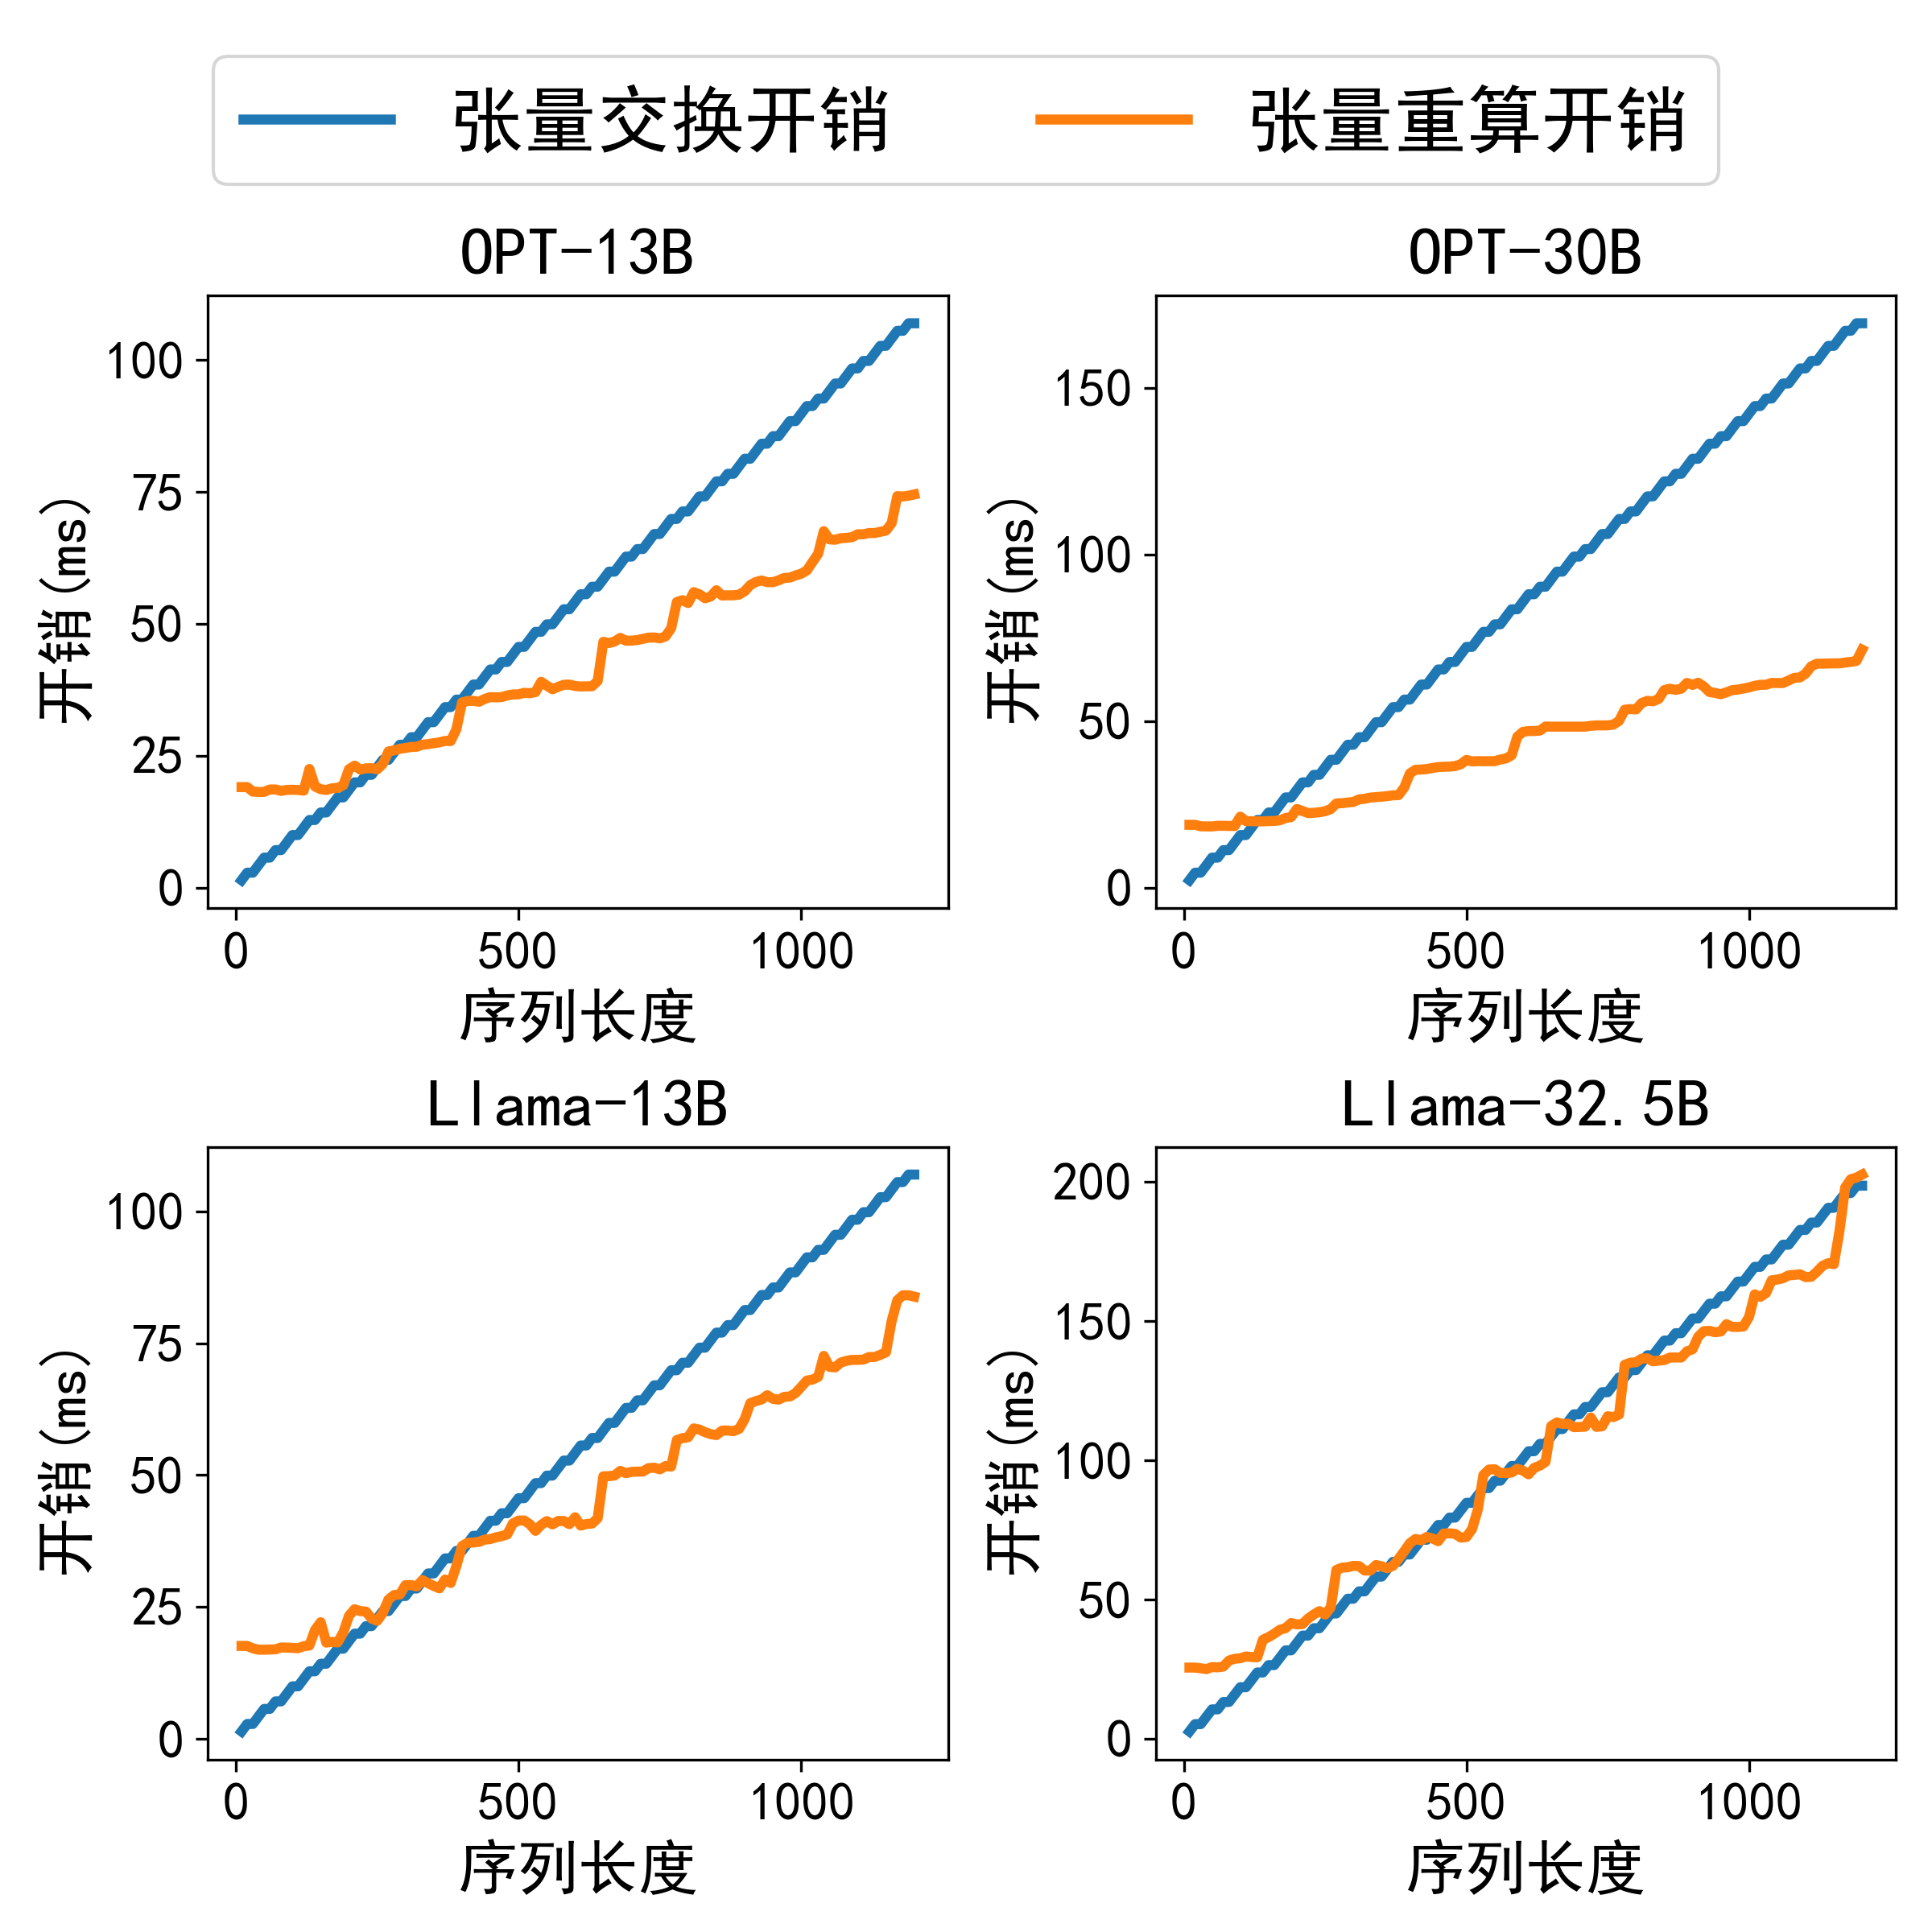
\includegraphics[width=0.85\linewidth]{交换与重算开销对比.png}
    \caption{交换与重算开销对比}
    \label{Fig:交换与重算开销对比}
  \end{figure}

\begin{itemize}    
    \item \textbf{张量重算开销}:自注意力机制内核采用并行计算策略,每个线程只计算一个token的qkv张量及注意力值。随着序列长度的增长,线程数量增加,同步开销随之上升,而单线程计算量不变,导致张量重算开销随序列长度增加呈亚线性增长。
    \item \textbf{张量交换开销}:KV Cache保存每个token的key-value张量,其内存占用与序列长度呈正比关系,而PCIe传输带宽在推理过程中基本保持稳定。因此张量交换开销与序列长度也呈正比关系。
\end{itemize}

因此,张量重算开销随序列长度的增长速度小于张量交换开销。在贪心采样策略下,对于长序列而言,无论是vLLM还是AdaptiveLLM,都使用张量重算,两种策略带来内存优化行为没有差异。对于短序列而言,vLLM使用张量重算,而AdaptiveLLM使用开销较小的张量交换,此时能够带来整体吞吐率提升。且OPT-13B和Llama-13B相比于OPT-30B和Llama-32.5B,在序列长度较短时,张量交换相比于张量重算,开销优势更加明显。

在LLM实际应用场景中,大多数序列的长度较短,使得张量交换在提升性能上拥有明显优势。而当长序列较多,或者CPU内存空间不足时,张量重算技术能够发挥优势。AdaptiveLLM能够基于服务器软硬件环境、LLM与数据集选取、用户参数设置与推理任务运行时信息来精准预测张量交换与张量重算开销,并选择开销较小的内存优化技术执行。 

  \section{AdaptiveLLM的设计与实现}

本章介绍了本文工作的具体设计。第一节给出AdaptiveLLM的整体设计方案, 后面的章节将分别介绍AdaptiveLLM中不同的功能模块。

\subsection{整体架构}

AdaptiveLLM实现了三个主要功能模块,包括张量重算开销分析器、张量交换开销分析器和自适应LLM推理优化器,其整体架构如图\ref{Fig:整体设计架构}所示。

\begin{figure}[!htbp]
  \centering
  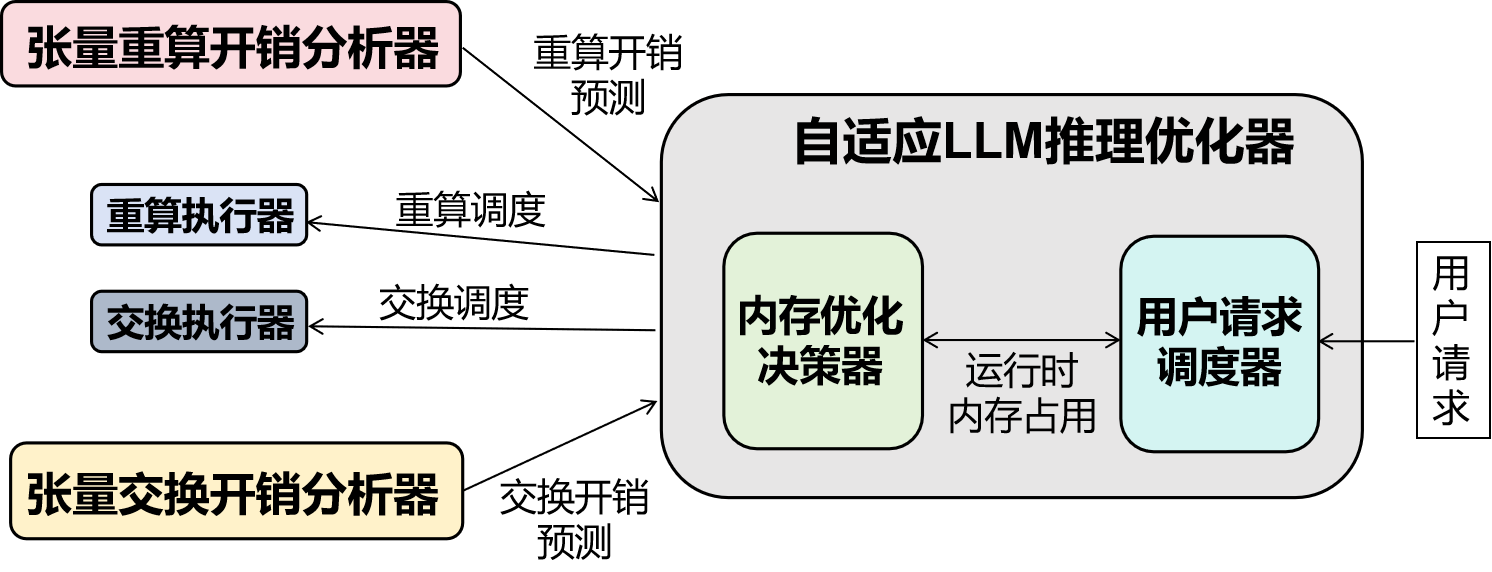
\includegraphics[width=0.9\linewidth]{整体设计架构.png}
  \caption{整体设计架构}
  \label{Fig:整体设计架构}
\end{figure}

张量重算开销分析器基于序列长度、模型隐藏维度、模型层数和批处理大小来预测重算开销。张量交换开销分析器基于KV Cache内存占用和GPU-CPU双向传输带宽来预测交换开销。自适应LLM推理优化器包含内存优化决策器和用户请求调度器。当GPU内存不足时,内存优化决策器引入基于开销感知的内存优化策略,选择优先级最低的用户请求,收集张量重算开销分析器与张量交换开销分析器提供的开销预测值。选择开销小的内存优化方式,而后交付相应的执行器。该过程称为“抢占调度”。当GPU内存空余时,用户请求调度器使用基于公平性的用户请求调度策略,在满足公平性的前提下尽可能多地调度剩余用户请求,避免GPU资源浪费。该过程称为“启动调度”。在推理过程中,内存优化决策器与用户请求调度器共享KV Cache内存占用信息。二者高效协同,实现整体吞吐率与单请求延时的权衡。

\subsection{张量重算开销分析器}

抢占调度时,重算执行器在内存中删除用户请求的KV Cache张量。启动调度时,执行一次prefill阶段来恢复被删除的数据。因此,张量重算引入的额外开销等于被抢占请求执行prefill阶段的时间。

本文以OPT和Llama模型为例,通过算子粒度复杂度分析来识别单步推理时间的影响因素。

\subsubsection{算子粒度开销分析}

OPT和Llama模型中包含5种不同的算子:ReLU、Norm、Linear、SiluAndMul和Attention,其计算流程如图\ref{Fig:四种算子的计算流程}所示。图中$X_i$,$Y_i$是由用户输入决定的张量维度;$input\_dim$,$output\_dim$,$head\_size$是由算子本身决定的张量维度。 

\begin{figure}[!htbp]
  \centering
  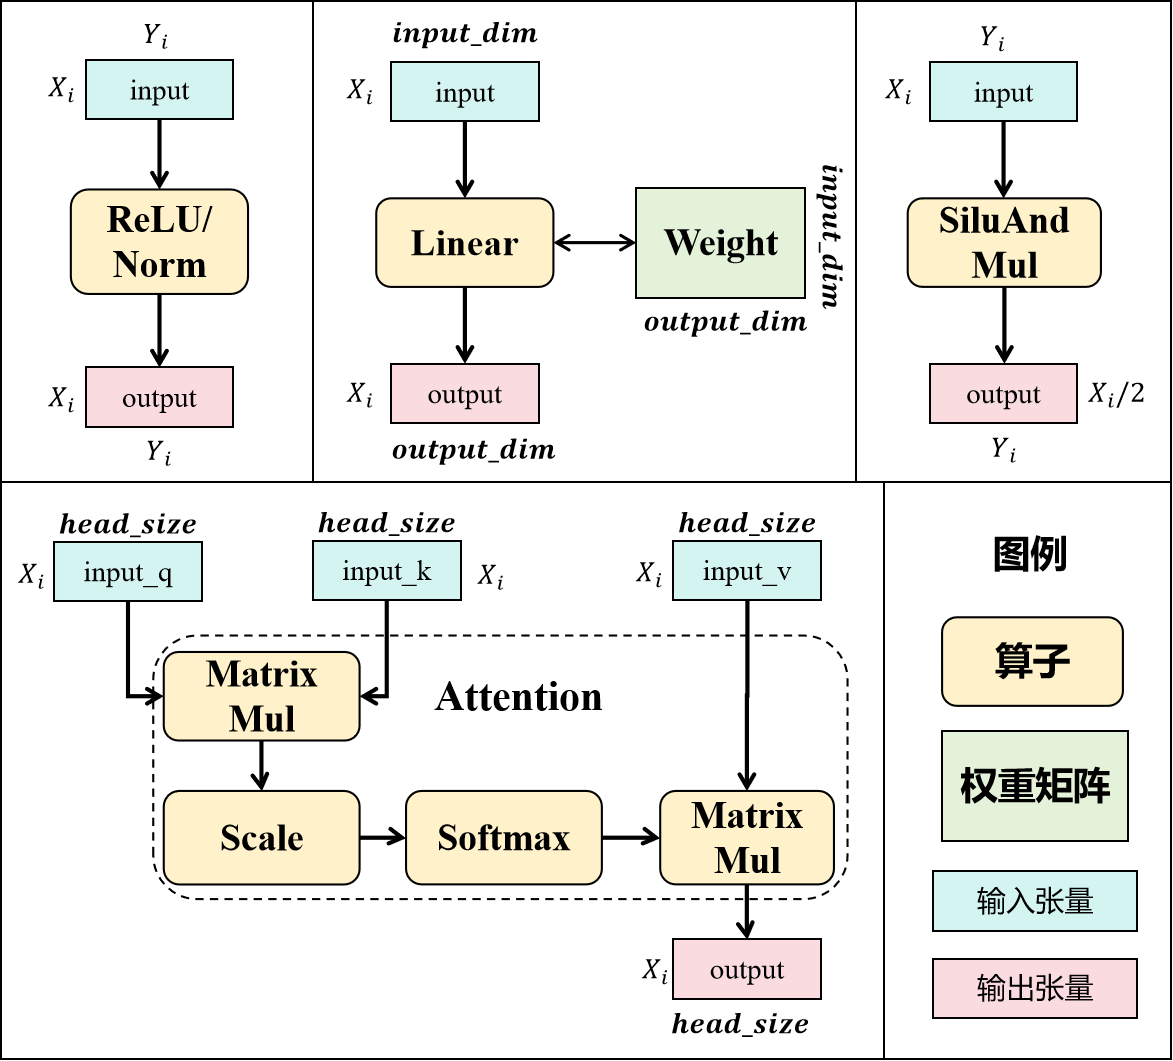
\includegraphics[width=0.9\linewidth]{四种算子的计算流程.png}
  \caption{四种算子的计算流程}
  \label{Fig:四种算子的计算流程}
\end{figure}

下面分别对这些算子进行复杂度分析。

\begin{itemize}
  
  \item \textbf{ReLU算子}:逐位调用激活函数进行计算,其时间复杂度为$O(X_i*Y_i)$。
  
  \item \textbf{Norm算子}:是LayerNorm、RMSNorm(仅在Llama模型中)等多种归一化算子的统称,其时间复杂度为$O(X_i*Y_i)$。
  
  \item \textbf{Linear算子}:将输入向量从$input\_dim$维空间映射到$output\_dim$维空间中,其计算复杂度为$O(X_i*input\_dim*output\_dim)$。
  
  \item \textbf{SiluAndMul算子}:该算子仅出现在Llama模型的MLP层中,将输入向量的指定维度减半,其时间复杂度为$O(X_i*Y_i)$。
  
  \item \textbf{Attention算子}:属于复合操作,由矩阵乘法、缩放和Softmax激活等底层算子组成,整体计算过程如公式\ref{Eq:Attention},其时间复杂度为$O(X_i^2*head\_size)$。
  \begin{equation}
    \small
    Attention(Q,K,V)=softmax(\frac{Q\times K^T}{\sqrt{h}}\times V)
    \label{Eq:Attention}
  \end{equation}

\end{itemize}

根据算子粒度复杂度分析,可以识别出4项有关LLM单步推理执行时间的影响因素,分别为:LLM层数、LLM隐藏维度、单请求需要处理的token数量、和批处理大小。

\subsubsection{单步推理开销预测模型}

单步迭代执行时间预测是一项拥有4个输入变量,1个输出变量的回归预测任务。根据算子粒度时间复杂度分析可知,输出变量与输入变量之间存在多项式依赖关系。因此,本文共选用了8个回归模型,包括线性回归模型、决策树回归模型、随机森林回归模型、岭回归模型、套索回归模型、弹性回归模型、梯度提升回归模型、和K-临近回归模型。针对每种回归模型,对不同的多项式拟合次数(1到10)进行测试。选择在测试集上预测误差最小的配置,并将其部署到AdaptiveLLM的张量重算开销分析器中。 

\subsection{张量交换开销分析器}

抢占调度时,交换执行器将用户请求的KV Cache从GPU传输到CPU中(换出阶段)。启动调度时,将其KV Cache传输回GPU中(换入阶段)。因此,张量交换引入的额外开销等于被抢占请求的换出时间与换入时间之和。

换出开销与换入开销的计算方式如公式\ref{Eq:Swap Overhead}所示。

\begin{equation}
  \begin{aligned}
    SwapOut\_Time=\frac{KVCach\_Mem}{DtoH-bandwidth} \\
    SwapIn\_Time=\frac{KVCache\_Mem}{HtoD-bandwidth}
  \end{aligned}
  \label{Eq:Swap Overhead}
  \setlength{\abovedisplayskip}{0ex}
  \setlength{\belowdisplayskip}{2ex}
\end{equation}

其中$DtoH-bandwidth$是数据从GPU传输到CPU的带宽,$HtoD-bandwidth$是数据从CPU传输到GPU的带宽。AdaptiveLLM继承了vLLM所采用的Paged Attention技术,在GPU和CPU内存中划分大小固定的Block,用于存储KV Cache。每个Block的内存占用如公式\ref{Eq:Block Mem}所示,其中$block\_size$是用户定义的参数,用于调整Block大小。

\begin{equation}
  \begin{aligned}
    block\_mem = 2 \times num\_layers \times hidden\_size \\ 
    \times block\_size \times sizeof(float16)
  \end{aligned}
  \label{Eq:Block Mem}
  \setlength{\abovedisplayskip}{0ex}
  \setlength{\belowdisplayskip}{2ex}
\end{equation}

因此,假设一个用户请求的长度为$n$,占用GPU block的数量为$block\_num$,则其KV Cache占用的总内存空间如公式\ref{Eq:KV Cache Mem}所示。

\begin{equation}
  \begin{aligned}
    KVCache = block\_mem \times block\_num  \\ =  block\_mem \times \lceil \frac{n}{block\_size} \rceil
  \end{aligned}
  \label{Eq:KV Cache Mem}
  \setlength{\abovedisplayskip}{0ex}
  \setlength{\belowdisplayskip}{2ex}
\end{equation}

由此可以计算出张量交换引入的额外开销。在上述公式中,换入换出传输带宽是由实验环境所决定的,在传输数据量较大时基本保持稳定。而$block\_size$与$block\_mem$在推理任务中均保持不变。因此对于不同的用户请求,其区别仅在于序列长度$n$的不同。

%wsq 抢占方式就是内存优化方式?是的话统一下用词
\subsection{内存优化决策器}

当GPU内存不足时,需要调用内存优化策略。AdaptiveLLM中的内存优化策略分为张量交换和张量重算两种。根据上文的分析,张量交换引入的额外开销等于KV Cache的换出开销与换入开销之和;张量重算引入的额外开销等于prefill过程的开销。\par

\begin{algorithm}
  \caption{Mem\_Schedule}
  \label{Code:内存优化决策器工作流程}
  \small
  \begin{spacing}{1.1}
    \begin{algorithmic}[1]
      \REQUIRE {运行队列$r$, 重算兼等待队列$w$, 交换队列$s$} 
      \ENSURE {无}
      \STATE {$sorted(r, key=<priority>, order=asc)$}
      \WHILE{$require\_mem(r) > avail\_gpu\_mem()$}
        \STATE {$req\gets r.pop()$} \hfill {// 优先级最低的用户请求}
        \STATE {$recomp\_time \gets GET\_RECOMP\_TIME(req)$}
        \STATE {$swap\_time \gets GET\_SWAP\_TIME(req)$}
        \IF {$swap\_time < recomp\_time \land \newline 
          kv\_cache\_mem(req) \leq avail\_cpu\_mem()$}
          \STATE {$SWAP(req)$} \hfill {// 交付张量交换执行器}
          \STATE {$s.append(req)$} \hfill {// 进入交换队列}
        \ELSE
          \STATE {$RECOMP(req)$} \hfill {// 交付张量重算执行器}
          \STATE {$w.append(req)$} \hfill {// 进入重算兼等待队列}
        \ENDIF
      \ENDWHILE
    \end{algorithmic}
  \end{spacing}
\end{algorithm}

张量交换和张量重算带来的额外开销成为阻拦用户请求并发度进一步提升的瓶颈,因此内存优化方式的选择尤为重要。在不同的运行环境中,应该使用不同的内存优化策略,减少额外开销。然而,vLLM在内存优化策略的选择上并未考虑开销问题。针对使用贪心采样策略的用户请求,其执行张量重算。针对使用并行采样或束搜索采样策略的用户请求,其执行张量交换。因此在面对GPU内存瓶颈时难以有效地压缩开销,进而无法提升吞吐率。AdaptiveLLM则对两种内存优化方式的开销进行比较,选择更优者执行。内存优化决策器的工作流程如算法\ref{Code:内存优化决策器工作流程}所示。

当剩余的GPU内存空间不足以存放运行队列在下一次迭代中产生的KV Cache时(第2行),内存优化决策器进入工作状态。选择运行队列中优先级最低的用户请求(第3行),调用张量交换开销分析器和张量重算开销分析器来预测其张量交换和张量重算开销(第4、5行)。如果交换开销小于重算开销,则该请求进入交换队列,并交付交换执行器处理(第6-8行);否则进入重算队列,并交付重算执行器处理(第9-11行)。以上过程循环执行,直至运行队列在下一次迭代中产生的KV Cache能够全部存放到GPU内存中。 此外,当CPU内存不足时,内存优化决策器将直接调用张量重算技术(第6行)。

%wsq 算两个开销前加个if判断,可以给个注释解释在干啥,如果内存不足直接选重算。两行完事儿?加一下吧
%此外,当CPU内存不足时,内存优化决策器将直接调用张量重算,而跳过开销预测和比较过程。

\subsection{用户请求调度器}

AdaptiveLLM维护三个用户请求队列:$waiting$队列、$running$队列与$swapped$队列。$waiting$队列存储初次进入调度系统,还未执行过,或者因张量重算而失去KV Cache的用户请求;$running$队列存储正在运行(执行decode阶段)的用户请求;$swapped$队列存储被换出到CPU中的用户请求。这三个队列之间拥有以下调度规则:

\begin{itemize} 

  \item $running$队列中的用户请求运行完毕后会返回客户端,否则继续运行。

  \item 当GPU内存空余时,$swapped$队列中的用户请求可以直接转移至$running$队列中。

  \item 当GPU内存空余时,$waiting$队列中的用户请求可以在执行prefill阶段后转移至$running$队列。

\end{itemize}

如果剩余的GPU内存空间不足以存储$running$队列在下一次迭代中产生的KV Cache,则需要内存优化决策器进行抢占调度。如果剩余的GPU空间足够,则执行启动调度,以扩充$running$队列,避免浪费GPU资源。用户请求调度器将部分请求从$swapped$队列或$waiting$队列中转移至$running$队列中。但由于两种转移方式存在较大差别(是否需要执行prefill阶段),因此每次扩充$running$队列时,或者仅从$swapped$队列进行调度,或者仅从$waiting$队列进行调度,而无法同时调度两个队列。用户请求调度器的工作流程如算法\ref{Code:用户请求调度器工作流程}所示。

\begin{algorithm}
  \caption{Req\_Schedule}
  \label{Code:用户请求调度器工作流程}
  \small
  \begin{spacing}{1.1}
    \begin{algorithmic}[1]
      \REQUIRE {大模型$LLM$}, {待执行的用户请求队列$L$}
      \ENSURE {无}
      \STATE {$w\gets L$}  \hfill {// 初始化waiting队列}
      \STATE {$r\gets empty\_list$} \hfill {// 初始化running队列}
      \STATE {$s\gets empty\_list$} \hfill {// 初始化swapped队列}
      \WHILE {$\neg (w.is\_empty()\land s.is\_empty() \land r.is\_empty())$}
        \STATE {$MemSchedule(r, w, s)$}  \hfill {// (内存不足时)抢占调度}
        \STATE {$s\_sche\gets SWAP\_IN\_SCHE()$}  \hfill {// 换入队列构建}
        \STATE {$w\_sche\gets RECOMP\_SCHE()$}  \hfill {// 重算队列构建}
        \IF {$GET\_PRI(w\_sche)\leq GET\_PRI(s\_sche)$}
          \STATE {$r=r+s\_sche$}  \hfill {// 换入}
          \STATE {$s=s-s\_sche$}
        \ELSE
          \STATE {$LLM.PREFILL(w\_sche)$}  \hfill {// 重算}
          \STATE {$r=r+w\_sche$}  
          \STATE {$w=w-w\_sche$}          
          \STATE \textbf{continue}
        \ENDIF
        \STATE {$LLM.DECODE(r)$} \hfill {// 单次推理迭代}
        \STATE {$r \gets [req \in r | \lnot req.is\_finished()]$} \hfill {// 移除完成的请求}
      \ENDWHILE
    \end{algorithmic}
  \end{spacing}
\end{algorithm}

客户端发送的用户请求进入$waiting$队列中,而$running$队列和$swapped$队列最初为空(第1-3行)。当GPU内存不足时,调用内存优化算法进行抢占调度(第5行),否则执行启动调度。 \par

用户请求调度器尽可能多地寻找能从$swapped$队列转移至$running$队列的用户请求(第6行),和能从$waiting$队列转移至$running$队列的用户请求(第7行)。对它们进行优先级比较(第8行),若前者的优先级均值较高,则将其直接转移到$running$队列中(第9-10行);若后者的优先级均值较高,则其执行prefill阶段后转移至$running$队列中,同时直接进入下一轮迭代(第12-15行)。需要注意的是,当GPU内存不足时,无法实现从$swapped$队列或$waiting$队列向$running$队列的调度,即$w\_sche$和$s\_sche$队列均为空,也就不存在后续的优先级比较过程了。 \par

在以上调度操作完成后,$running$队列应当为非空的,否则推理过程无法继续。$running$队列执行decode阶段作为本次迭代(第17行),将已完成的用户请求移除后进入下一次迭代(第18行)。 \par

对于一个用户请求,定义其优先级等于处理时间除以序列长度,其中处理时间等于当前时刻减去该用户请求初次进入$waiting$队列的时刻。定义用户请求队列的优先级等于所有用户请求优先级的平均值。当用户请求初次进入$waiting$队列时,其序列长度较短,优先级增长较为迅速,能够被很快处理。而在等待过程中,其优先级在不断提升,避免了饥饿现象。 \par

% wsq 这一段可以扔到实验分析里,分析为啥vllm差(如果后面实验部分没写的话),方法里不要写。
% vLLM基于FCFS策略进行设计,在调度时优先考虑$swapped$队列,只有当$swapped$队列为空时才调度$waiting$队列,使得以交换方式被抢占的用户请求相比于以重算方式被抢占的用户请求,其重调度的优先级更高。结合上一小节关于vLLM固定式抢占策略的分析可知,一部分用户请求被抢占后能够很快重新调度,而也有一部分用户请求被抢占后进入$waiting$队列的末位,需要长时间等待。这种调度策略违反了公平性原则。本文中的用户请求调度器基于公平性原则而设计,同时在实验部分证明,其能够大幅提升用户请求的实时性。
  \section{实验验证}

本章介绍实验部分。第一节为实验平台软硬件配置。第二节介绍LLM模型与数据集选取,以及实验参数设置。第三节针对基于开销感知的内存优化策略,进行吞吐率测试。第四节针对基于公平性的用户请求调度策略,进行实时性测试。第五节分析张量交换与张量重算预测误差。第六节进行其它测试工作。

\subsection{实验环境}

本文开展实验使用的服务器软硬件配置如表\ref{Table:实验平台的软硬件配置}所示。使用Intel(R) Xeon(R) CPU和NVIDIA A800 80GB GPU作为硬件环境,使用CUDA-11.8、PyTorch-2.0.l和vLLM-0.2.5作为底层框架进行开发。服务器使用PCIe连接实现GPU-CPU通信。

\begin{table}[H]
  \centering
  \caption{实验平台的软硬件配置}
  \label{Table:实验平台的软硬件配置}
  \renewcommand{\arraystretch}{1.15}
  \small
  \begin{tabular}{c c}
    \toprule
    \textbf{软件/硬件} & \textbf{型号/版本} \\ 
    \midrule
    CPU & Intel(R) Xeon(R) CPU @ 2.60GHz  \\ 
    GPU & NVIDIA A800 PCIE 80GB \\ 
    OS & CentOS Linux 7 (Core) \\ 
    CUDA & 11.8 \\ 
    PyTorch & 2.0.1 \\ 
    vLLM & 0.2.5 \\ 
    \bottomrule
  \end{tabular}
\end{table}

% 服务器使用PCIe连接实现GPU-CPU通信。PCIe传输带宽在传输数据量不同时差异显著,表\ref{Table:PCIe双向传输带宽}列出了部分情况。在计算张量交换开销时,需要根据单次实际传输的数据量(一般是一个Block或其中的一部分)找到对应的传输带宽值。

% \begin{table}[H]
%   \centering
%   \caption{PCIe双向传输带宽}
%   \label{Table:PCIe双向传输带宽}
%   \renewcommand{\arraystretch}{1.2}
%   \small
%   \begin{tabular}{c c c}
%     \toprule
%     \textbf{传输量(B)} & \textbf{HtoD(MB/s)} & \textbf{DtoH(MB/s)} \\
%     \midrule
%     1024 & 0.19 & 0.24 \\ 
%     2048 & 0.60 & 0.72 \\ 
%     4096 & 1.20 & 1.49 \\ 
%     8192 & 1.07 & 2.97 \\ 
%     16384 & 4.16 & 5.79 \\ 
%     32768 & 7.76 & 9.35 \\ 
%     102400 & 14.27 & 16.49 \\ 
%     204800 & 18.30 & 20.24 \\ 
%     409600 & 21.17 & 22.57 \\ 
%     \bottomrule
%   \end{tabular}
% \end{table}

\begin{figure*}[!htbp]
  \centering
  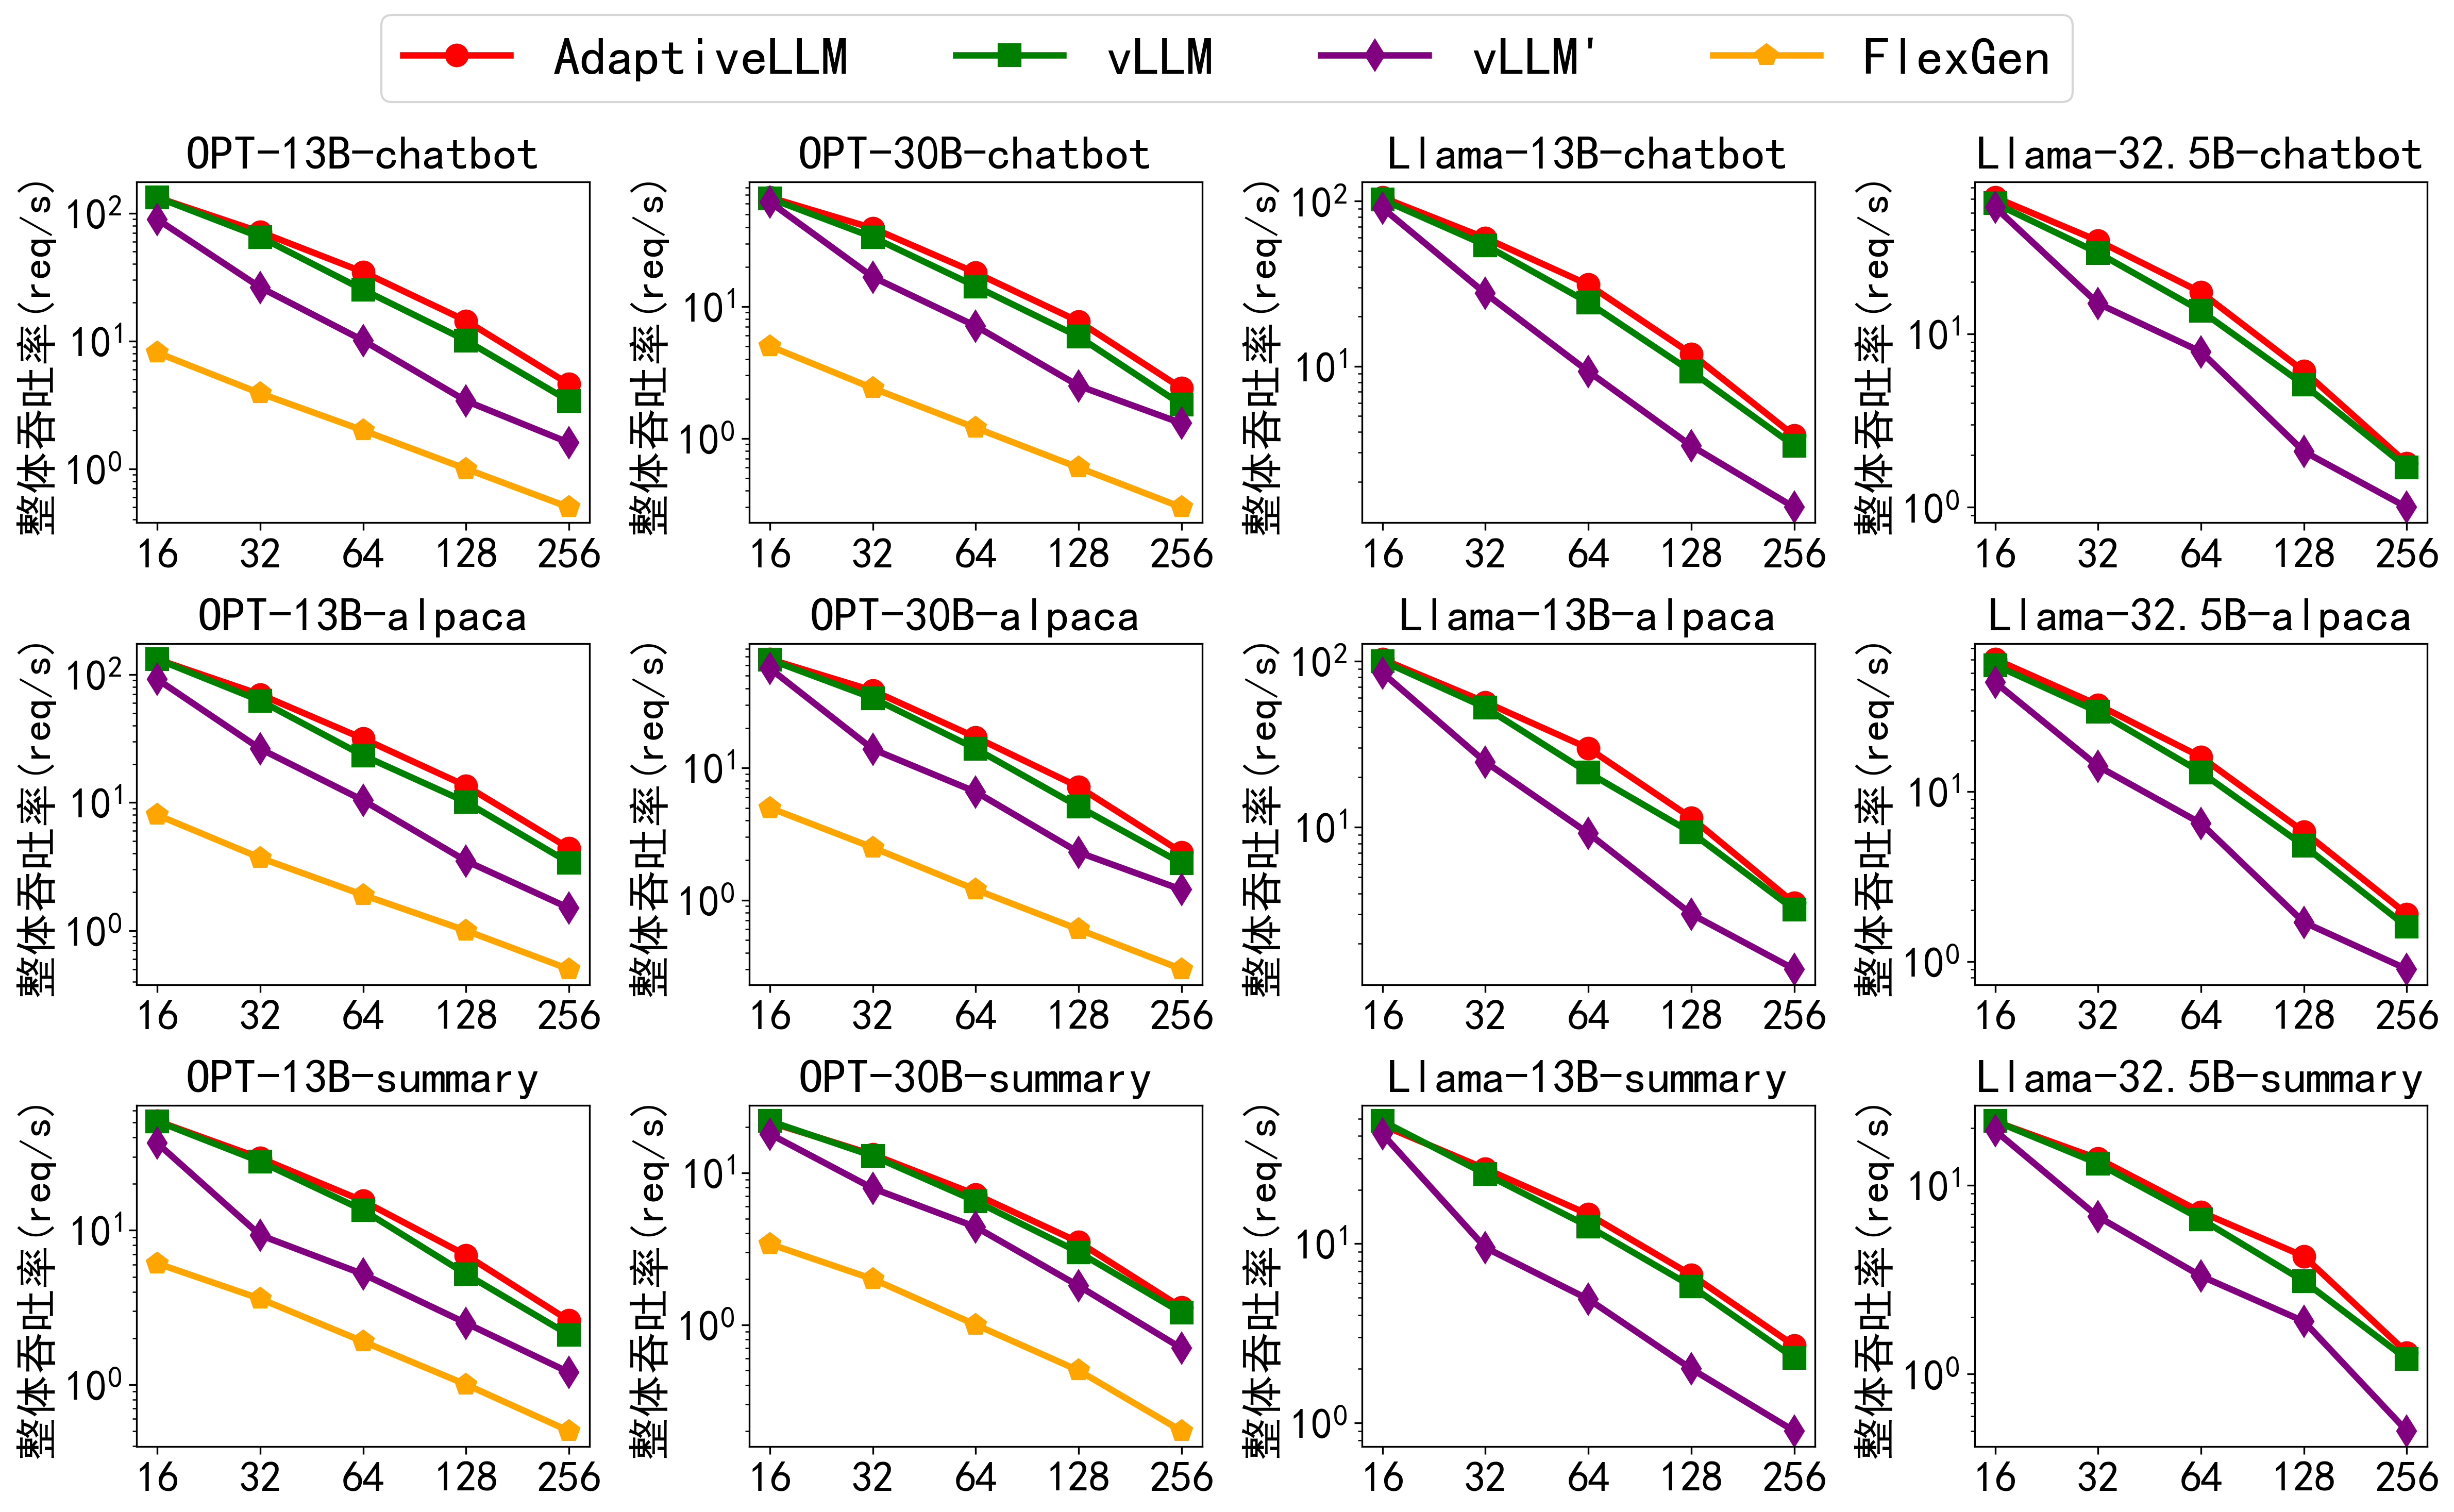
\includegraphics[width=0.85\linewidth]{推理任务吞吐率.png}
  \caption{推理任务吞吐率}
  \label{Fig:推理任务吞吐率}
\end{figure*}

\subsection{模型与数据集}

本文选用OPT~\cite{OPT}(OPT-13B、OPT-30B)和Llama~\cite{Llama}(Llama-13B、Llama-32.5B)作为实验模型,在三个常见数据集(Chatbot~\cite{Chatbot}、Alpaca~\cite{Alpaca}、Summary~\cite{Summary})上进行测试。数据集信息如表\ref{Table:实验数据集选取}所示。

\begin{table}[H]
  \centering
  \caption{实验数据集选取}
  \label{Table:实验数据集选取}
  \renewcommand{\arraystretch}{1.15}
  \small
  \begin{tabular}{c c c c}
    \toprule
    \textbf{数据集} & \textbf{样本总数} & \textbf{平均输入长度} & \textbf{任务类型} \\
    \midrule
    Chatbot & 258064 & 17.02 & 对话类 \\
    Alpaca & 68912 & 19.66 & 指令类 \\
    Summary & 1799 & 340.48 & 摘要类 \\
    \bottomrule
  \end{tabular}
\end{table}

Chatbot和Alpaca中大多数序列长度较短,而Summary中序列长度展现出很大差异性,且包含长序列。它们涵盖了LLM应用程序面临的大部分场景。

实验过程中的参数设置模拟LLM应用程序在多任务并发场景下的运行状态。{\color{red} 具体来说,本文将GPU Block数量设置为128,以保证抢占调度在GPU内存不足时得以发生;将CPU Block数量设置为64,以避免内存优化决策器简单地将部分序列交付张量交换执行器。}针对12个实验组,在相应数据集中使用简单随机抽样法选取1000个样本进行后续测试。

%wsq 实验部分改一下顺序,重要的实验放前面。吞吐率测试,实时性测试,执行时间预测,开销分析。

% wsq 这应该算是motivation实验,基于这个观察你才有空间去选择策略。不应该出现在大实验中。
% \subsection{重算与交换的开销对比}

% 本文对OPT-13B、OPT-30B、Llama-13B和Llama-32.5B进行开销对比测试,其结果如图\ref{Fig:交换与重算开销对比}所示。当序列长度较小时,交换开销小于重算开销;随着序列长度的增加,二者大小关系反转。原因如下:  \par

% 自注意力机制内核采用并行计算策略,每个线程只计算一个token的qkv张量及注意力值。随着token数量增多,并行执行的线程数量增加,线程间同步开销随之上升,而单线程计算量不变。因此张量重算开销随序列长度增加呈亚线性增长。而由公式\ref{Eq:Swap Overhead}、\ref{Eq:Block Mem}、\ref{Eq:KV Cache Mem}可知,张量交换开销与序列长度呈近似正比关系。因此,张量重算开销的增长速度小于张量交换开销。  \par

% \begin{figure}[!htbp]
%   \centering
%   \includegraphics[width=0.9\linewidth]
%   {交换与重算开销对比.png}
%   \caption{交换与重算开销对比}
%   \label{Fig:交换与重算开销对比}
% \end{figure}

% 在贪心采样策略下,对于长序列(如Summary数据集中的部分样本),无论是vLLM还是AdaptiveLLM,都偏向于使用重算,两种策略带来的抢占行为没有差异。对于短序列(如Chatbot和Alpaca数据集),vLLM使用重算,而AdaptiveLLM使用开销较小的交换,此时能够带来吞吐率提升。在LLM实际应用场景中,大多数序列的长度较短,使得张量交换在提升性能上拥有明显优势。而当长序列较多,或者CPU内存空间不足时,张量重算技术能够发挥优势。 

\subsection{吞吐率测试}

本文以vLLM作为基准框架,针对AdaptiveLLM进行吞吐率测试。{\color{red}由于本文在推理过程中使用贪心采样策略来生成新token,因此vLLM内存管理器在GPU内存不足时固定调用张量重算技术。同时,对vLLM框架稍加修改形成vLLM$\_$s,使其固定调用张量交换技术。}图\ref{Fig:推理任务吞吐率}展示了12个实验组在推理任务中的整体吞吐率测试结果,其横坐标为序列最大输出长度。表\ref{Table:AdaptiveLLM相对于基准框架的加速比}给出了最大输出长度为64时,AdaptiveLLM相对于vLLM和vLLM$\_$s的具体加速比。结果表明,相比于vLLM和vLLM$\_$s基准框架,AdaptiveLLM实现了最高1.40$\times$和2.55$\times$的整体吞吐加速。

%wsq 论文中每一句都要对自己的工作有正向意义,这句只暴露了自己的弊端
由于Summary数据集的平均序列长度和方差均明显高于Alpaca和Chatbot数据集,因此在相同条件下,其推理吞吐率低于Alpaca和Chatbot。尽管如此,与vLLM相比,AdaptiveLLM在Summary数据集上也达到了1.1$\times$加速比。

\begin{table}[H]
  \centering
  \caption{AdaptiveLLM相对于基准框架的加速比}
  \label{Table:AdaptiveLLM相对于基准框架的加速比}
  \renewcommand{\arraystretch}{1.15}
  \small
  \begin{tabular}{c c c c}
    \toprule
    \textbf{LLM-数据集} & \textbf{Chatbot} & \textbf{Alpaca} & \textbf{Summary} \\
    \midrule
    OPT-13B	& 1.38/2.46 & 1.36/2.55 & 1.15/2.50 \\
    OPT-30B	& 1.27/1.98 & 1.22/1.99 & 1.11/1.64 \\
    Llama-13B & 1.28/2.28 & 1.40/2.37 & 1.17/2.12 \\
    Llama-32.5B & 1.28/1.95 & 1.23/2.13 & 1.09/2.18 \\
    \bottomrule
  \end{tabular}
\end{table}

AdaptiveLLM可以根据模型配置,灵活地选择合适的内存优化策略。CPU内存的限制使vLLM$\_$s的批处理大小低于vLLM和AdaptiveLLM,因此吞吐率较低。当序列最大输出长度限制在较低水平时,每个请求执行推理任务所需的迭代次数较少,资源需求量低,抢占鲜有发生,此时AdaptiveLLM和vLLM的性能差距不大。随着最大输出长度的增加,有限的GPU内存无法满足需求,AdaptiveLLM调用基于开销感知的内存优化策略,展现性能优势。当最大输出长度过大时,无论是AdaptiveLLM还是vLLM,其批处理大小均限制在较低水平,但AdaptiveLLM仍具有明显优势(当序列最大输出长度为256时,AdaptiveLLM在vLLM的基础上实现最高1.3$\times$的加速比)。

在Chatbot和Alpaca数据集的推理任务中,序列长度较短,批处理大小高。根据预测器给出的结果可知,此时张量交换开销小于张量重算开销。然而随着新token的不断生成,大量用户请求需要被换出,导致CPU内存不足。因此AdaptiveLLM执行了大量张量交换操作和少量张量重算操作。

在Summary数据集的推理任务中,其序列长度较大,批处理大小低。张量交换发生频率较低,极少出现CPU内存不足的现象,此时张量重算操作的执行大部分来源于开销比较的结果。

综上所述,在基于开销感知的内存优化策略下,AdaptiveLLM在GPU内存不足时预测张量交换与张量重算开销,并选择开销较小的内存优化技术执行,进而大幅度提升推理任务整体吞吐率。 

\begin{figure*}[!htbp]
  \centering
  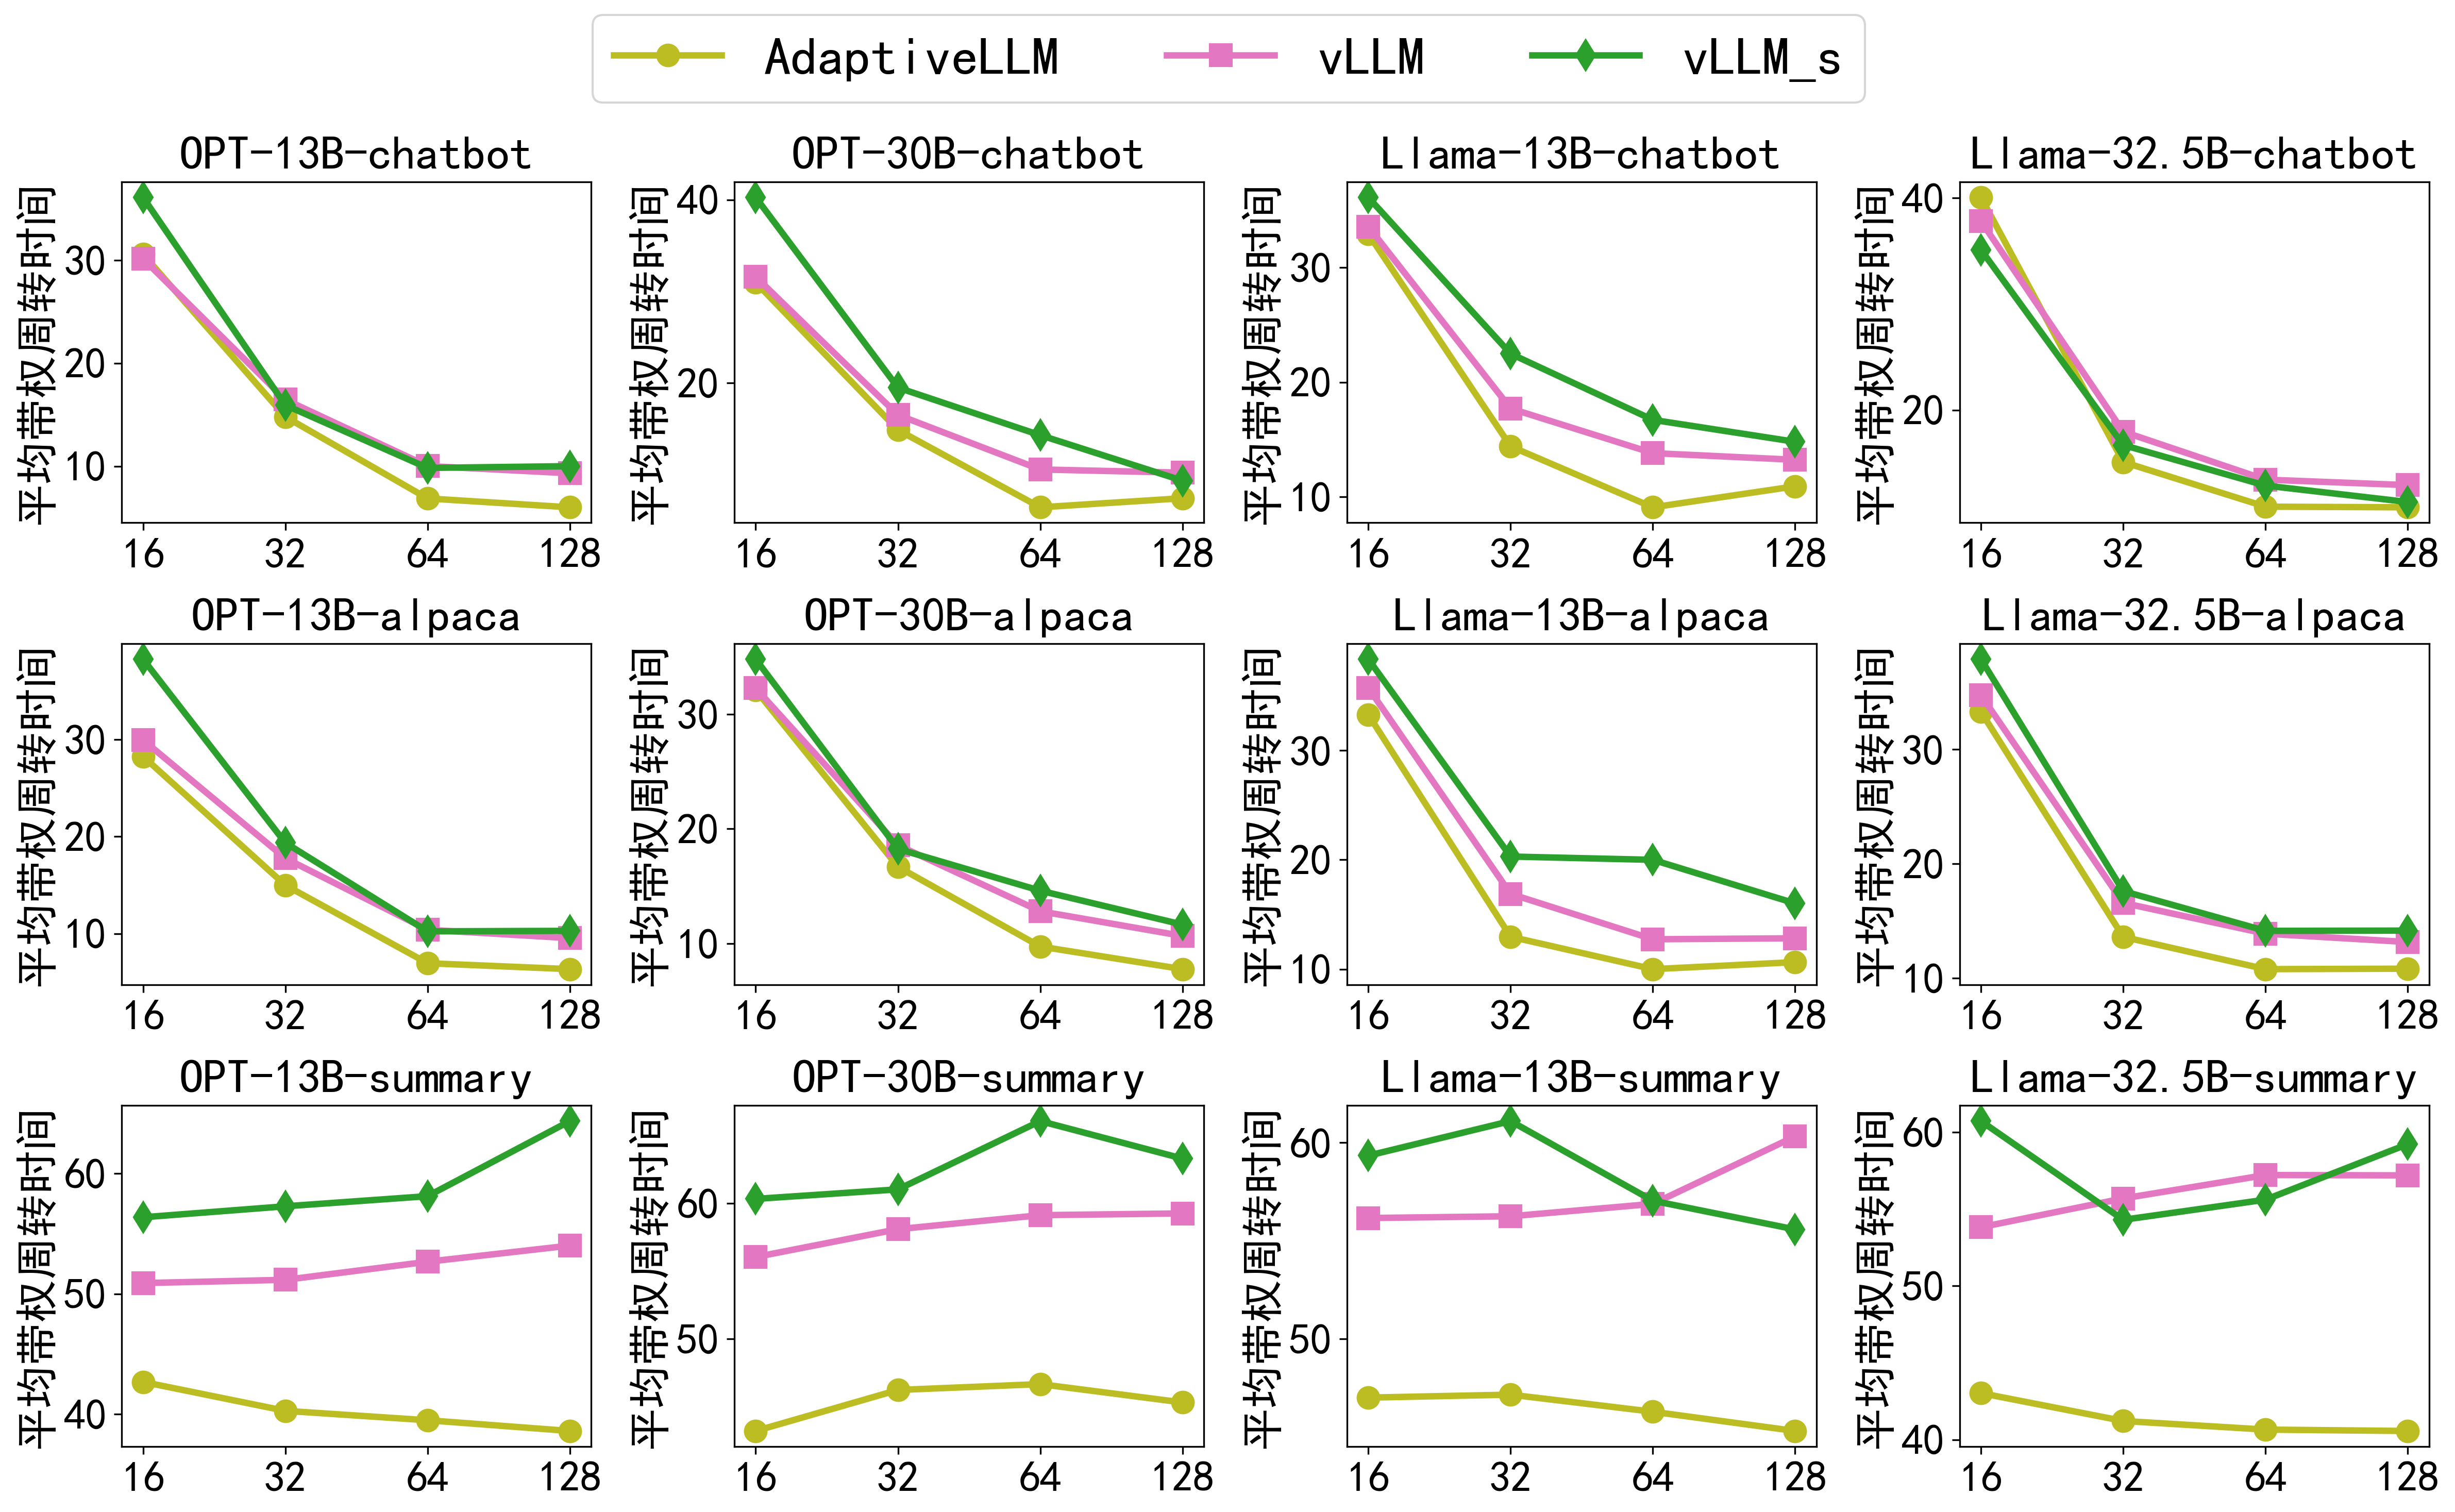
\includegraphics[width=0.85\linewidth]{用户请求平均带权周转时间.png}
  \caption{用户请求平均带权周转时间}
  \label{Fig:平均带权周转时间}
\end{figure*}

\subsection{实时性测试}

%wsq 公式中需要说明各个变量都是什么
为了消除整体吞吐率变化对实时性测试的影响,本文选取平均带权周转时间作为测试指标。用户请求带权周转时间等于客户端响应时间除以服务器端处理时间,如公式\ref{Eq:Weighted Around Time}所示。对于某一用户请求来说,$finish\_t$是其处理完毕时刻,$send\_t$是其从客户端发送至服务器端的时刻,$sche\_t$是其被AdaptiveLLM初次调度的时刻。平均带权周转时间($\geq 1$)越低,说明用户请求处理过程中的排队时间占比越低。 

\begin{equation}
  \begin{aligned}
    w\_around\_t = \frac{finish\_t - send\_t}{finish\_t - sche\_t}
  \end{aligned}
  \label{Eq:Weighted Around Time}
  \setlength{\abovedisplayskip}{0ex}
  \setlength{\belowdisplayskip}{2ex}
\end{equation}

%wsq 阐述一下和vllm_s的比较结果。此外图片中vllm's改成vllm_s

图\ref{Fig:平均带权周转时间}展示了平均带权周转时间随批处理大小上限的变化情况。在不同批处理大小设置下,基于公平性的用户请求调度策略均能使平均带权周转时间显著下降。当批处理大小较大时(64或128),AdaptiveLLM的平均带权周转时间相比于vLLM下降了20\%至40\%,相比于vLLM$\_$s下降了20\%至60\%。

对于序列较短的Chatbot和Alpaca数据集而言,随着批处理大小的上升,GPU利用更加充分,因此平均带权周转时间下降。在实际运行中,当批处理大小到达64至128时,GPU产生内存瓶颈,此时批处理大小无法继续提升,平均带权周转时间达到最小值。

对于序列较长的Summary数据集而言,其处理并发度被限制在较低水平(10以下),无法达到用户设置的批处理大小上限。因此平均带权周转时间呈稳定状态。AdaptiveLLM中高效的调度策略展现优势,使用户请求等待时间显著低于vLLM和vLLM\_s。

综上所述,基于公平性的用户请求调度策略使得用户请求从客户端发送至服务器端后能够很快开始处理,不会出现长时间等待现象。

\subsection{预测误差测试}

\subsubsection{张量重算预测误差}

张量重算开销由张量重算开销分析器根据LLM层数、LLM隐藏维度、单请求需要处理的token数量、以及批处理大小预测得到。本文分别测试了OPT模型和Llama模型单步推理执行时间的预测效果。OPT执行时间预测任务共有6.4w条训练数据和1.6w条测试数据,结果表明,随机森林回归模型性能最佳,其在拟合2次多项式时能够达到1.76\%的预测误差。Llama执行时间预测任务有6.8w条训练数据和1.7w条测试数据,结果表明,随机森林模型同样性能最佳,其在拟合2次多项式时能够达到1.30\%的预测误差。

% \subsection{其它测试}

% wsq 合并到前面
\subsubsection{张量交换预测误差}

张量交换预测开销由张量交换开销分析器根据用户请求的KV Cache内存占用和GPU-CPU双向传输带宽而计算得到。本文针对模型Llama-13B和Llama-32.5B进行测试,其结果如图\ref{Fig:交换开销预测误差}所示。两个模型换入开销预测的MAPE误差分别为1.5\%和1.1\%,换出开销预测的MAPE误差分别为1.0\%和1.2\%。因此,张量交换开销总预测误差低于4\%。

\begin{figure}[!htbp]
  \centering
  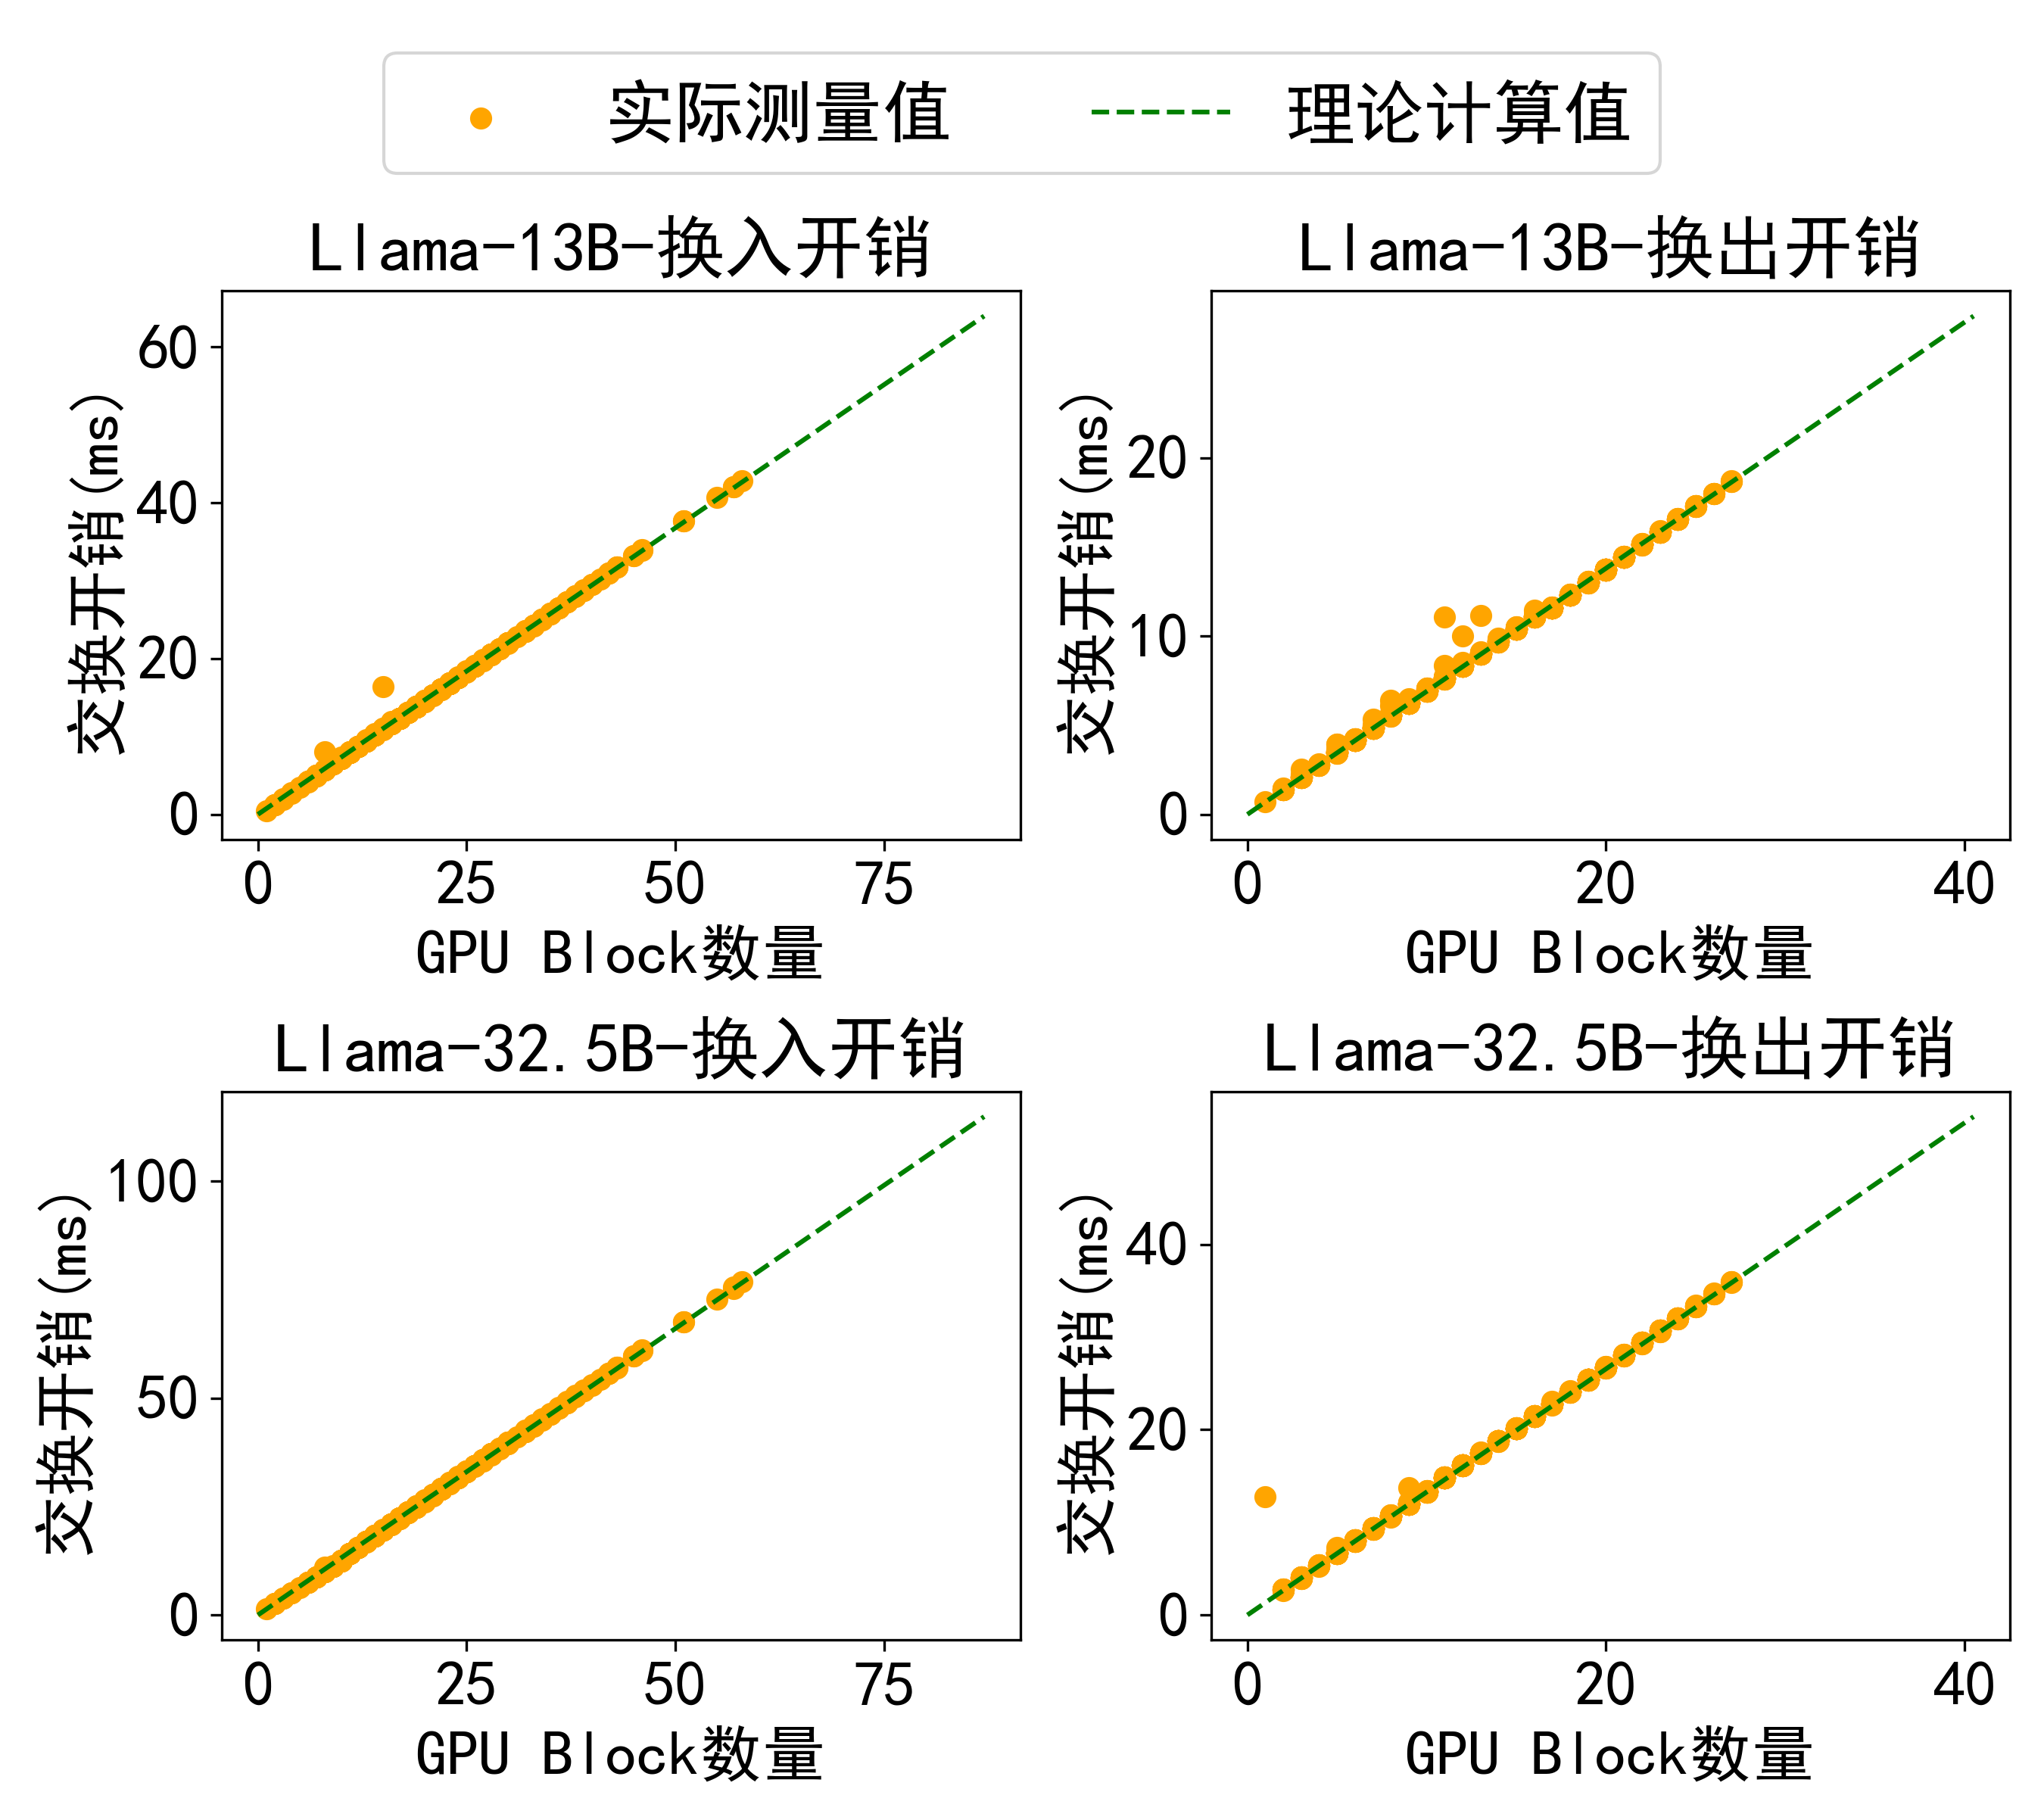
\includegraphics[width=0.85\linewidth]{交换开销预测误差.png}
  \caption{交换开销预测误差}
  \label{Fig:交换开销预测误差}
\end{figure}

\subsection{开销测试}

基于开销感知的内存优化策略在获取张量重算和张量交换开销时,会带来新的预测开销。本文设计如下对照实验获取预测过程的开销:在吞吐率测试过程中,当GPU内存不足时调用开销比较过程,但最终使用vLLM提供的固定式内存优化策略(张量重算)。观察此情景下推理任务的总用时可知,预测开销在推理任务中仅占0.1\%至1\%。

{\color{red}基于公平性的用户请求调度策略也有一定的开销。理论上,该算法的时间复杂度为$O(r^2)$,其中$r$为running队列中用户请求的数量。在实际运行过程中,每次调度的开销在0.2ms左右,总开销在推理任务中仅占0.5\%至1\%。综上所述,AdaptiveLLM引入的两种优化策略所带来的额外开销均可忽略不计。}

  \section{相关工作}

%wsq 参考学术paper的相关工作格式,将相关工作分为几类介绍。
\subsubsection{张量交换技术}
%wsq 总分总 参考mimose 中间列举4-5个工作 最后总结 大概写法:之前工作swapping关注activation 本文关注进一步关注到了kvcache并做了精细建模

随着批处理大小的增加或模型参数量的扩展,运行时需要保存的张量会超出GPU的内存限制。张量交换技术在GPU空间不足时开启,将一部分需要保存,而暂时用不到的张量换出至CPU中,在计算需要时重新换入GPU中。

HuggingFace Accelerate~\cite{Huggingface-Accelerate}实现了张量交换技术,但换出与换入的张量仅限于LLM的参数张量。LightLLM~\cite{LightLLM}能够针对KV Cache进行张量交换,但换出的比例设计为定值,无法根据运行时信息调整。

FlexGen~\cite{Swapping}首次提出了“自适应内存优化”的概念,通过线性规划建模在交换方案的可行域内进行搜索,在给定的时间内找到较优解。然而,FlexGen假设运行队列中的所有用户请求拥有相同的输出长度。在实际情况下,输出长度具有很大的差异性,使得相关理论无法推广。

本文针对KV Cache实现张量交换技术,并进行细粒度内存占用建模分析。根据GPU内存使用水平,进行实时换出换入调整。

\subsubsection{张量重算技术}
%同上

Mimose~\cite{Recomputation}等工作提出了张量重算技术。在抢占式用户请求调度系统中,当某个请求获得执行权时,会检查之前的计算结果是否保存在GPU中,如果不在,则需要重新获取这部分计算结果。此时可以无需将之前存储的计算结果(如果有)从CPU或磁盘中换入到GPU中,而仅仅对它们进行重新计算。

对于执行LLM推理任务的用户请求而言,这些key-value张量在初次生成时经历了多次前向传播,而在重算过程中仅需调用自注意力机制即可得到,因此张量重算的开销远远小于token序列初次生成时的开销,不会导致计算量的爆炸式增长。

{\color{red}Capuchin~\cite{Capuchin}提出张量交换和张量重算的开销预测方法,且首次对二者的选择开展深入研究。然而,其优化技术仅面向DNN训练场景,针对前向传播到反向传播之间需要保存的中间张量实现。面向LLM推理场景下的张量优化技术仍有待深入分析。}

\subsubsection{LLM推理优化技术}
%结构同上 列举几个工作如orca 最后总结 大概写法:和那些方法正交

除了张量交换和张量重算等针对张量层面的优化策略以外,传统LLM推理框架还采用了很多其他推理优化技术。

ORCA~\cite{ORCA}将批处理调度的粒度从单个用户请求细化为单次推理迭代,化解了用户请求相互等待的性能瓶颈。vLLM~\cite{vLLM}基于OS页式内存管理思想,在ORCA的基础上引入Paged Attention机制。vLLM相比于OCRA,大幅度提升显存利用率,增加批处理大小上限,进而提升推理任务的整体吞吐率。

SpecInfer~\cite{SpecInfer}引入了投机推理技术(Speculative Sampling),根据小型LLM的输出来预测大型LLM的输出,在大幅度提升推理吞吐率的同时保障了输出质量。DistillSpec~\cite{DistillSpec}在SpecInfer的基础上实现了知识蒸馏技术(Knowledge Distillation,KD),使得输出预测的准确率显著提升。

本文提出的LLM推理优化策略能够与调度粒度细化、投机推理等研究工作相兼容。本文设计了规范且友好的用户接口,开发者能够根据任务需求来定义各种参数,极大地方便了有关推理优化的深入研究。

% \subsubsection{\color{red}{早期工作}}

% Hugging Face Accelerate~\cite{Huggingface-Accelerate}实现了张量交换技术,但换出与换入的张量仅限于LLM的参数张量。DeepSpeed ZeRO-Inference~\cite{GPT-175B资源消耗}实现了LLM的分布式推理,能够利用数据并行性与张量并行性来实现LLM推理加速。但以上两个框架均无法针对KV Cache实现张量交换技术,也没有实现张量重算。
  
% \subsubsection{\color{red}{张量交换的提出}}

% FlexGen~\cite{Swapping}首次提出了“自适应内存优化”的概念,并将张量交换的范围由参数张量扩展至所有张量。通过线性规划建模在交换方案的可行域内进行搜索,在给定的时间内找到较优解。同时,FlexGen还实现了张量压缩技术,相比于Hugging Face Accelerate和DeepSpeed ZeRO-Inference,实现了较大的吞吐率提升。然而,FlexGen假设运行队列中的所有用户请求拥有相同的输出长度。在实际情况下,输出长度具有很大的差异性,使得相关理论无法推广。
  
% \subsubsection{\color{red}{调度粒度的转变}}

% ORCA~\cite{ORCA}将批处理调度的粒度从单个用户请求转化为单次推理迭代,化解了用户请求相互等待的性能瓶颈。vLLM~\cite{vLLM}在ORCA的基础上实现了张量重算技术。基于OS页式内存管理思想,引入Paged Attention机制来实现。vLLM相比于OCRA,大幅度提升显存利用率,并增加批处理大小上限,进而提升推理任务的整体吞吐率。同时,vLLM设计了规范且友好的用户接口,开发者能够根据任务需求来定义各种参数,极大地方便了有关推理优化的深入研究。
  
% \subsubsection{\color{red}{投机推理技术}}

% SpecInfer~\cite{SpecInfer}引入了投机推理技术(Speculative Sampling),根据小型LLM的输出来预测大型LLM的输出,在大幅度提升推理吞吐率的同时保障了输出质量。DistillSpec~\cite{DistillSpec}在SpecInfer的基础上实现了知识蒸馏技术(Knowledge Distillation,KD),使得输出预测准确率显著提升。

  \section{未来工作}

本文将针对以下部分进一步完善AdaptiveLLM框架。

\subsubsection{张量压缩技术}

有限的PCIe传输带宽使数据的GPU-CPU传输带来无法忽略的通信开销。随着LLM参数量和批处理大小的增加,通信开销成为主要性能瓶颈。近期工作中~\cite{Swapping},张量压缩技术常与张量交换技术联合使用,通过矩阵变换等数学方式减少传输参数量。高效的压缩技术能够在不损失张量精度的前提下减小通信开销,进一步提升批处理大小上限,提升吞吐率。

\subsubsection{内存优化与前向传播的并行}

\begin{itemize}

  \item \textbf{张量交换与前向传播的并行}:张量交换的本质是GPU-CPU通信传输过程,而前向传播的本质是GPU计算过程。二者在传统模式下串行执行。AdaptiveLLM计划在内存优化决策器中设计一个交换线程和一个计算线程,并行完成两项任务,进一步减少张量交换带来的额外开销。

  \item \textbf{张量重算与前向传播的并行}:SARATHI~\cite{SARATHI}框架研发了chunk-prefill技术,实现prefill阶段与decode阶段共置运行。由于张量重算的本质是prefill过程,因此若将该技术移植到AdaptiveLLM中,可以实现张量重算与前向传播的并行。

\end{itemize}

\subsubsection{张量并行与流水线并行~\cite{Parallelism}} AdaptiveLLM目前仅针对张量并行度与流水线并行度均为1的场景进行优化,本文将在未来实现张量并行技术与流水线并行技术。
  \section{结论}

本文设计了AdaptiveLLM,一款基于张量交换和张量重算的LLM推理服务框架。AdaptiveLLM实现了张量重算开销预测与张量交换开销预测,其预测误差分别在2\%和4\%以下。AdaptiveLLM研发了基于开销感知的张量优化策略和基于公平性的用户请求调度策略。基于开销感知的张量优化策略用于在GPU内存不足时,执行开销较小的抢占方式来保证推理任务的顺利完成;基于公平性的用户请求调度策略则能够在GPU内存充足时重新调度被抢占的用户请求。实验表明,相比于vLLM框架,AdaptiveLLM有10\%-40\%的整体吞吐率提升,实现了服务器端的处理加速;且AdaptiveLLM能够以合理的方式调度用户请求,将平均带权周转时间优化为vLLM的60\%~80\%,减少等待时间,实现了面向客户端的实时请求处理。综上所述,AdaptiveLLM权衡整体吞吐率与单请求延时,化解二者在优化实现上的矛盾。
  \bibliographystyle{gbt7714-numerical}
  \bibliography{references}
\end{document}